% Provenance (never printed): see sources/outline_sources.md (Year 1: the wind-driven
% circulation, gyres, Ekman transport and upwelling, western boundary currents, the
% meridional overturning circulation and the water masses). Exercise and problem values in
% the Book 3 scratch calculator calc/ch29.py; figures from figdata/bachelor-1/
% ekman_hodograph.py (Ekman's solution with Ekman's constants) and stommel_gyre.py
% (Stommel's 1948 model, exercise parameters), the world map from figdata/shared/geo.py.
% Physics owns the Coriolis force (recalled). Book 1 (g8) gave the surface currents and
% the gyres in words, Book 2 (g10) upwelling: re-founded here with the Ekman balance.
% Ch. 26 owns the T-S diagram and the water masses, ch. 28 the Coriolis parameter, the
% geostrophic wind and the mean meridional streamfunction. The Sverdrup balance, the
% vorticity argument and the derivation of the Ekman spiral are the Year 3 volume's; ENSO
% the Year 2 volume's.
\chapter{महासागर का परिसंचरण}\label{ch:b1:ocean-circulation}

1992 में, उत्तरी प्रशांत में एक तूफ़ान के दौरान, हाँगकांग से संयुक्त राज्य की ओर जाते एक जहाज़ से एक कंटेनर समुद्र में गिर गया। वह टूट गया और लगभग \num{29000} रबर की बत्तखें और अन्य स्नान-खिलौने छोड़ गया, जो तैरते हुए दूर-दूर तक निकल गए; जहाँ उनमें से कुछ बाद में मिले, उन्होंने वैज्ञानिकों को उन धाराओं को समझने में मदद की जो उन्हें ले गई थीं। तैरते खिलौने सतही जल का अनुसरण करते हैं, और महासागरों का सतही जल बेतरतीब नहीं भटकता: वह बेसिन-भर के गायरों में घूमता है, महासागरों के पश्चिमी तटों के साथ संकरी धाराओं में उत्तर की ओर दौड़ता है, और कुछ चुने हुए स्थानों पर ऊपर उठता या नीचे डूबता है। यह अध्याय समझाता है कि पवन ऊपरी महासागर को गति कैसे देती है, जल उस पवन के समकोण पर क्यों चलता है जो उसे धकेलती है, सबसे प्रबल धाराएँ महासागरों की पश्चिमी ओर से क्यों सटी रहती हैं, और एक मंद पलटाव जल को गहराई तक कैसे ले जाता है और वापस लाता है।
% ledger: noaa:floatees

\begin{omfigure}
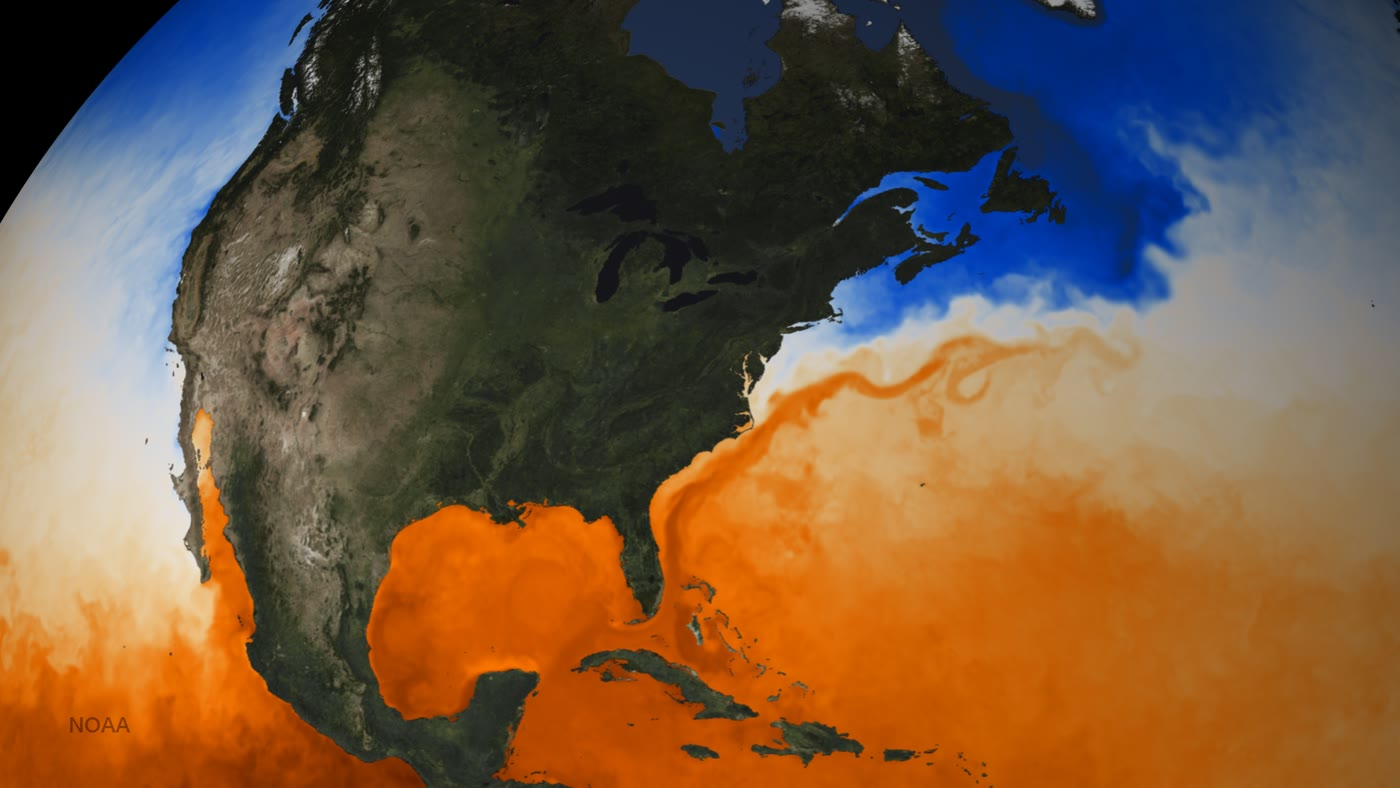
\includegraphics[width=0.85\linewidth]{images/book3/b1-gulf-stream-sst.jpg}

{\small 2016 के जून के आरंभ में उत्तरी अमेरिका के आसपास समुद्र-सतह का तापमान, उपग्रह आँकड़ों से (गरम पानी नारंगी, ठंडा पानी नीला)। खाड़ी धारा संयुक्त राज्य के तट से एक गरम, टेढ़ी-मेढ़ी फ़ीते-जैसी धारा के रूप में निकलती है और अटलांटिक पार यूरोप की ओर जाती है; उन्हीं अक्षांशों पर, प्रशांत तट के पास का पानी अटलांटिक तट के पास के पानी से कहीं ठंडा है। (फ़ोटो: NOAA, NESDIS, सार्वजनिक डोमेन, विकिमीडिया कॉमन्स के माध्यम से।)}
\label{fig:b1:ocean-circulation:sst}
\end{omfigure}
% ledger: commons:gulf-stream-sst, noaa:gulf-stream-heat

\begin{recall}
भौतिकी खंड कोरिऑलिस बल देते हैं। \Cref{ch:b1:atmospheric-circulation} ने उसका क्षैतिज भाग लिखा: $-f\,\vec k\times\vec v$, \omterm{def:b1:atmospheric-circulation:coriolis-parameter}{कोरिऑलिस प्राचल}
$f = 2\Omega\sin\varphi$ ($\Omega = \qty{7.292e-5}{rad.s^{-1}}$) के साथ, और उसने \omterm{def:b1:atmospheric-circulation:winds}{व्यापारिक पवनें}, भूमध्य रेखा और लगभग \ang{30} के बीच पूर्वी पवनें, और उसके आगे \omterm{def:b1:atmospheric-circulation:winds}{पछुआ पवनें} पाईं; उसने एक पलटाव के \omterm{def:b1:atmospheric-circulation:streamfunction}{माध्य उत्तर-दक्षिण धारा-फलन} को भी परिभाषित किया। \Cref{ch:b1:fluid-envelopes-structure} ने \omterm{def:b1:fluid-envelopes-structure:ocean-layers}{मिश्रित परत} और \omterm{def:b1:fluid-envelopes-structure:ocean-layers}{ताप-सीमा-परत}, समुद्री जल का घनत्व, T--S आरेख और दक्षिणी अटलांटिक के \omterm{def:b1:fluid-envelopes-structure:ts-diagram}{जल-द्रव्यमान} दिए, और \cref{ch:b1:radiation-heat-transport} ने वायुमंडल और महासागर द्वारा साझा किया गया ध्रुवोन्मुखी ऊष्मा परिवहन। पुस्तक~1 ने सतही धाराओं और महान गायरों का वर्णन किया; पुस्तक~2 ने कुछ तटों के साथ ठंडे जल के \omterm{def:b1:ocean-circulation:upwelling}{उत्सर्पण} का।
% ledger: earth:Trot, nos:gyres
\end{recall}

\section{पवन और सतही धाराएँ}\label{sec:b1:ocean-circulation:wind}

पवन समुद्र को उस पर रगड़ कर गति देती है। उसका बल सतह पर फैला होता है, और उसे दाब की तरह, प्रति इकाई क्षेत्र मापा जाता है।

\begin{definition}[पवन-प्रतिबल]\label{def:b1:ocean-circulation:wind-stress}
\emph{पवन-प्रतिबल}\index{पवन-प्रतिबल} $\vec T$ प्रति इकाई क्षेत्र वह क्षैतिज बल है जो पवन समुद्र-सतह पर लगाती है, पास्कल में। यह वायु के क्षैतिज संवेग का महासागर में नीचे की ओर स्थानांतरण है, और लगभग पवन की दिशा में इंगित करता है। उसका परिमाण थोक सूत्र से दिया जाता है:
\[
  T = \rho_a C_D U_{10}^2,
\]
जहाँ $\rho_a = \qty{1.3}{kg.m^{-3}}$ वायु का घनत्व है, समुद्र के \qty{10}{m} ऊपर की पवन-गति $U_{10}$ और $C_D$ एक विमाहीन खिंचाव-गुणांक।
\end{definition}
% ledger: stewart:wind-stress

खिंचाव-गुणांक तेज़ यंत्रों से मापा जाता है जो लहरों के कुछ मीटर ऊपर पवन के विक्षुब्ध उतार-चढ़ाव दर्ज करते हैं। तटस्थ रूप से स्थिर वायु के लिए, येलैंड और टेलर के मापन देते हैं:
\[
  1000\,C_D = 0.29 + \frac{3.1}{U_{10}} + \frac{7.7}{U_{10}^2}
  \quad (\qtyrange{3}{6}{m/s}),
  \qquad
  1000\,C_D = 0.60 + 0.071\,U_{10}
  \quad (\qtyrange{6}{26}{m/s}),
\]
$U_{10}$ मीटर प्रति सेकंड में। \qty{10}{m/s} की पवन के लिए $C_D =
\num{1.31e-3}$ है और वह $T = 1.3 \times \num{1.31e-3} \times 100 =
\qty{0.170}{Pa}$ लगाती है; \qty{5}{m/s} की पवन, \qty{0.040}{Pa}; \qty{20}{m/s} की आँधी, \qty{1.05}{Pa}। पवन को \qty{10}{m/s} से \qty{20}{m/s} तक दोगुना करने पर
प्रतिबल $6.2$ गुना होता है, $4$ गुना नहीं: खुरदरे समुद्र पवन को अधिक कसकर पकड़ते हैं। ये प्रतिबल नगण्य हैं, वायुमंडलीय दाब के दस लाखवें भाग जितने, पर वे पूरे महासागर पर बिना रुके कार्य करते हैं।
% ledger: stewart:drag-coefficient (computed in figdata/bachelor-1/ekman_hodograph.py and calc/ch29.py)

प्रतिबल का प्रतिरूप पवनों के प्रतिरूप का अनुसरण करता है। उष्णकटिबंधों की व्यापारिक पवनों, जो पश्चिम की ओर बहती हैं, और मध्य-अक्षांशों की पछुआ पवनों, जो पूर्व की ओर बहती हैं, के बीच हर महासागर बेसिन का सतही जल घूमने लगता है।

\begin{definition}[गायर; उपोष्णकटिबंधीय और उपध्रुवीय गायर]\label{def:b1:ocean-circulation:gyre}
एक \emph{गायर}\index{गायर} एक महासागर बेसिन को भरने वाली घूमती महासागरीय धाराओं की एक बड़ी प्रणाली है। एक \emph{उपोष्णकटिबंधीय गायर}\index{उपोष्णकटिबंधीय गायर} व्यापारिक पवनों और पछुआ पवनों के बीच होता है और उत्तरी गोलार्ध में दक्षिणावर्त और दक्षिणी में वामावर्त मुड़ता है। एक \emph{उपध्रुवीय गायर}\index{उपध्रुवीय गायर} पछुआ पवनों की ध्रुवीय ओर होता है और उलटी दिशा में मुड़ता है।
\end{definition}
% ledger: nos:gyre-def, nos:boundary-currents, stewart:north-atlantic

पाँच \omterm{def:b1:ocean-circulation:gyre}{उपोष्णकटिबंधीय गायर} हैं: उत्तरी और दक्षिणी अटलांटिक, उत्तरी और दक्षिणी प्रशांत और हिंद महासागर में; कोई भी भूमध्य रेखा के आर-पार नहीं फैलता। उत्तरी अटलांटिक में \omterm{def:b1:ocean-circulation:gyre}{उपोष्णकटिबंधीय गायर} पश्चिम में संयुक्त राज्य के तट के साथ खाड़ी धारा से और पूर्व में अफ़्रीका के पास कैनरी धारा से बंद होता है; उसके उत्तर में \omterm{def:b1:ocean-circulation:gyre}{उपध्रुवीय गायर} वामावर्त मुड़ता है, जिसकी दक्षिणी ओर उत्तरी अटलांटिक धारा है और पश्चिमी ओर लैब्रेडोर धारा दक्षिण की ओर बहती है। निम्न अक्षांशों पर अटलांटिक और प्रशांत की पश्चिम-वाही भूमध्यरेखीय धाराएँ एक पूर्व-वाही प्रति-धारा से अलग होती हैं। \omterm{def:b1:ocean-circulation:gyre}{गायर} सममित नहीं हैं: हर \omterm{def:b1:ocean-circulation:gyre}{उपोष्णकटिबंधीय गायर} अपने बेसिन की पश्चिमी ओर एक प्रबल, संकरी धारा से और पूर्वी ओर एक दुर्बल, चौड़ी धारा से बंद होता है। अंटार्कटिका के चारों ओर, जहाँ कोई महाद्वीप उसे नहीं रोकता, अंटार्कटिक परिध्रुवीय धारा विश्व के चारों ओर पूर्व की ओर बहती है, दक्षिणी महासागर की पछुआ पवनों से चलाई जाती हुई।
% ledger: nos:boundary-currents, stewart:north-atlantic, stewart:heat-conveyor, lien:kuroshio, donohue:acc, stewart:acc

\begin{omfigure}
\begin{tikzpicture}
\begin{axis}[ommap, width=0.98\linewidth, xtick={-180,-120,...,180}, ytick={-60,-30,0,30,60}]
% land: figdata/shared/geo.py; ledger: data:ne-land. Arrows placed by hand from the
% ledgered pattern: nos:boundary-currents, stewart:north-atlantic, lien:kuroshio,
% donohue:acc, stewart:acc
\addplot[fill=omLithAlluv, draw=black!45, line width=0.2pt, forget plot] table {figdata/out/shared-geo-land.dat};
% North Atlantic subtropical gyre (clockwise)
\addplot[omThm, line width=1.1pt, -{Stealth[length=4pt]}, smooth] coordinates {(-80,26) (-77,32) (-70,37) (-58,40) (-44,41)};
\addplot[omThm, line width=1.1pt, -{Stealth[length=4pt]}, smooth] coordinates {(-38,40) (-28,39) (-20,36)};
\addplot[omThm, line width=1.1pt, -{Stealth[length=4pt]}, smooth] coordinates {(-19,32) (-21,24) (-26,17)};
\addplot[omThm, line width=1.1pt, -{Stealth[length=4pt]}, smooth] coordinates {(-32,14) (-45,13) (-60,15)};
% North Atlantic subpolar gyre (anticlockwise)
\addplot[omDef, line width=1.1pt, -{Stealth[length=4pt]}, smooth] coordinates {(-40,47) (-28,52) (-18,57)};
\addplot[omDef, line width=1.1pt, -{Stealth[length=4pt]}, smooth] coordinates {(-24,61) (-35,62) (-44,59)};
\addplot[omDef, line width=1.1pt, -{Stealth[length=4pt]}, smooth] coordinates {(-55,59) (-56,53) (-51,47)};
% North Pacific subtropical gyre (clockwise)
\addplot[omThm, line width=1.1pt, -{Stealth[length=4pt]}, smooth] coordinates {(123,19) (125,26) (133,32) (143,36) (156,38)};
\addplot[omThm, line width=1.1pt, smooth] coordinates {(162,39) (172,40) (180,40.5)};
\addplot[omThm, line width=1.1pt, -{Stealth[length=4pt]}, smooth] coordinates {(-180,40.5) (-165,41) (-148,40)};
\addplot[omThm, line width=1.1pt, -{Stealth[length=4pt]}, smooth] coordinates {(-133,37) (-128,29) (-122,20)};
\addplot[omThm, line width=1.1pt, -{Stealth[length=4pt]}, smooth] coordinates {(-125,13) (-150,12) (-175,13)};
\addplot[omThm, line width=1.1pt, -{Stealth[length=4pt]}, smooth] coordinates {(170,13) (152,14) (135,15)};
% South Atlantic subtropical gyre (anticlockwise)
\addplot[omThm, line width=1.1pt, -{Stealth[length=4pt]}, smooth] coordinates {(2,-8) (-15,-9) (-30,-9)};
\addplot[omThm, line width=1.1pt, -{Stealth[length=4pt]}, smooth] coordinates {(-34,-14) (-39,-24) (-47,-34)};
\addplot[omThm, line width=1.1pt, -{Stealth[length=4pt]}, smooth] coordinates {(-42,-40) (-20,-40) (2,-38)};
\addplot[omThm, line width=1.1pt, -{Stealth[length=4pt]}, smooth] coordinates {(10,-31) (9,-23) (6,-15)};
% South Pacific subtropical gyre (anticlockwise)
\addplot[omThm, line width=1.1pt, -{Stealth[length=4pt]}, smooth] coordinates {(-88,-10) (-120,-11) (-160,-12)};
\addplot[omThm, line width=1.1pt, -{Stealth[length=4pt]}, smooth] coordinates {(160,-16) (157,-26) (162,-35)};
\addplot[omThm, line width=1.1pt, -{Stealth[length=4pt]}, smooth] coordinates {(-170,-40) (-140,-41) (-105,-39)};
\addplot[omThm, line width=1.1pt, -{Stealth[length=4pt]}, smooth] coordinates {(-82,-36) (-82,-27) (-85,-17)};
% Indian Ocean subtropical gyre (anticlockwise)
\addplot[omThm, line width=1.1pt, -{Stealth[length=4pt]}, smooth] coordinates {(98,-13) (80,-14) (60,-15)};
\addplot[omThm, line width=1.1pt, -{Stealth[length=4pt]}, smooth] coordinates {(47,-22) (40,-29) (33,-34)};
\addplot[omThm, line width=1.1pt, -{Stealth[length=4pt]}, smooth] coordinates {(50,-38) (75,-37) (100,-35)};
\addplot[omThm, line width=1.1pt, -{Stealth[length=4pt]}, smooth] coordinates {(108,-31) (106,-24) (102,-18)};
% Antarctic Circumpolar Current (eastward)
\addplot[omMeth, line width=1.4pt, -{Stealth[length=5pt]}, smooth] coordinates {(-62,-58) (-40,-55) (-15,-52)};
\addplot[omMeth, line width=1.4pt, -{Stealth[length=5pt]}, smooth] coordinates {(5,-52) (40,-50) (75,-50)};
\addplot[omMeth, line width=1.4pt, -{Stealth[length=5pt]}, smooth] coordinates {(95,-51) (130,-53) (165,-56)};
\addplot[omMeth, line width=1.4pt, -{Stealth[length=5pt]}, smooth] coordinates {(-170,-58) (-130,-59) (-85,-59)};
\node[font=\scriptsize, anchor=west, fill=white, fill opacity=0.8, text opacity=1, inner sep=1pt] at (axis cs:-66,31) {खाड़ी धारा};
\node[font=\scriptsize, anchor=west, fill=white, fill opacity=0.8, text opacity=1, inner sep=1pt] at (axis cs:-11,25) {कैनरी};
\node[font=\scriptsize, anchor=east, fill=white, fill opacity=0.8, text opacity=1, inner sep=1pt] at (axis cs:-58,52) {लैब्रेडोर};
\node[font=\scriptsize, anchor=west, fill=white, fill opacity=0.8, text opacity=1, inner sep=1pt] at (axis cs:142,28) {कुरोशियो};
\node[font=\scriptsize, anchor=north, fill=white, fill opacity=0.8, text opacity=1, inner sep=1pt] at (axis cs:-150,9) {उत्तरी भूमध्यरेखीय};
\node[font=\scriptsize, anchor=north, fill=white, fill opacity=0.8, text opacity=1, inner sep=1pt] at (axis cs:0,-62) {अंटार्कटिक परिध्रुवीय धारा};
\end{axis}
\end{tikzpicture}

{\small समुद्र-सतह के \omterm{def:b1:ocean-circulation:gyre}{गायर} (मानचित्र पर ज़मीन के ऊपर योजनाबद्ध तीर)। गहरा लाल: पाँच \omterm{def:b1:ocean-circulation:gyre}{उपोष्णकटिबंधीय गायर}, उत्तरी गोलार्ध में दक्षिणावर्त और दक्षिणी में वामावर्त, हर एक एक संकरी \omterm{def:b1:ocean-circulation:wbc}{पश्चिमी सीमा धारा} के साथ; नीला: उत्तरी अटलांटिक का \omterm{def:b1:ocean-circulation:gyre}{उपध्रुवीय गायर}; हरा: अंटार्कटिक परिध्रुवीय धारा। केवल पाठ में चर्चित धाराएँ नामित हैं। तीर प्रवाह की दिशा दिखाते हैं, गति नहीं।}
\label{fig:b1:ocean-circulation:gyres}
\end{omfigure}
% ledger: data:ne-land, nos:boundary-currents, stewart:north-atlantic, lien:kuroshio, donohue:acc

यह प्रतिरूप दो विशेषताओं की व्याख्या माँगता है। पहली घूर्णन की दिशा है: \omterm{def:b1:ocean-circulation:gyre}{उपोष्णकटिबंधीय गायर} की भूमध्यरेखीय ओर पर \omterm{def:b1:atmospheric-circulation:winds}{व्यापारिक पवनें} पश्चिम की ओर बहती हैं, फिर भी \omterm{def:b1:ocean-circulation:gyre}{गायर} की धाराएँ पवनों का सीधा अनुसरण नहीं करतीं, और सतही जल उनसे कोण पर बहता है। दूसरी असममिति है: \omterm{def:b1:ocean-circulation:gyre}{गायर} का वापसी प्रवाह अपने बेसिन की पश्चिमी ओर दबा दिया जाता है। दोनों पृथ्वी के घूर्णन से आते हैं।

\section{एकमान परिवहन}\label{sec:b1:ocean-circulation:ekman}

\begin{history}[नान्सेन और एकमान, 1898--1905]
आर्कटिक में अपनी यात्रा के दौरान, फ़्रिडटियोफ़ नान्सेन ने देखा कि पवन समुद्री बर्फ़ को पवन की दिशा में नहीं, बल्कि पवन की ओर देखते हुए अपने दाईं ओर, \ang{20} से \ang{40} के कोण पर धकेलती है। उसने तर्क दिया कि चलती बर्फ़ पर तीन बलों को संतुलित होना होगा: पवन का धक्का, पानी का घर्षण, और कोरिऑलिस बल। उसने मौसम-विज्ञानी विल्हेम बिएर्कनेस से कहा कि वे अपने एक छात्र को पवन-चालित धाराओं पर पृथ्वी के घूर्णन के प्रभाव का अध्ययन करने दें। वह छात्र, वॉल्फ़्रिड एकमान, ने उप्साला में अपनी डॉक्टरेट थीसिस के लिए सिद्धांत विकसित किया, और 1905 में उसका विस्तार किया। उसका हल आज भी पवन-चालित महासागर के सिद्धांत का आरंभिक बिंदु है।
\end{history}
% ledger: stewart:ekman-layer, nos:ekman-spiral

\begin{definition}[एकमान परत, एकमान परिवहन, एकमान सर्पिल]\label{def:b1:ocean-circulation:ekman}
\emph{एकमान परत}\index{एकमान परत} महासागर की पतली सतही परत है, अधिकतम कुछ सौ मीटर मोटी, जिसमें पवन का प्रतिबल प्रक्षुब्ध घर्षण द्वारा नीचे ले जाया जाता है और कोरिऑलिस बल द्वारा संतुलित होता है। \emph{एकमान परिवहन}\index{एकमान परिवहन} वह \omterm{def:b1:fluid-envelopes-structure:ts-diagram}{जल-द्रव्यमान} है जो परत प्रति सेकंड एक ऊर्ध्वाधर पट्टी के आर-पार ले जाती है जो \qty{1}{m} चौड़ी है, सतह से परत के नीचे तक:
\[
  \vec M = \int_{-d}^{0} \rho\,\vec v\,\mathrm dz \quad (\unit{kg.m^{-1}.s^{-1}});
\]
घनत्व से भाग देने पर, वह प्रति मीटर एक आयतन-परिवहन है, इकाई \unit{m^2.s^{-1}} में। \emph{एकमान सर्पिल}\index{एकमान सर्पिल} परत के भीतर गहराई के साथ धारा का घूमना और दुर्बल होना है। महासागर के परिवहन \emph{स्वर्डरप}\index{स्वर्डरप (इकाई)} में गिने जाते हैं: \qty{1}{\sverdrup} $=
\qty{e6}{m^3.s^{-1}}$।
\end{definition}
% ledger: stewart:ekman-layer, stewart:ekman-transport

\begin{theorem}[एकमान परिवहन]\label{thm:b1:ocean-circulation:ekman}
स्थायी अवस्था में, तटों से दूर, उस जल पर जो \omterm{def:b1:ocean-circulation:ekman}{एकमान परत} से कहीं गहरा है, \omterm{def:b1:ocean-circulation:ekman}{एकमान परिवहन} केवल \omterm{def:b1:ocean-circulation:wind-stress}{पवन-प्रतिबल} $\vec T$ और \omterm{def:b1:atmospheric-circulation:coriolis-parameter}{कोरिऑलिस प्राचल} $f$ पर निर्भर करता है:
\[
  \vec M = \frac{1}{f}\,\vec T\times\vec k,
  \qquad |\vec M| = \frac{|\vec T|}{|f|}.
\]
यह \omterm{def:b1:ocean-circulation:wind-stress}{पवन-प्रतिबल} के समकोण पर है, उत्तरी गोलार्ध में उसके दाईं ओर और दक्षिणी में बाईं ओर।
\end{theorem}
% ledger: stewart:ekman-transport

\begin{proof}
माना $\vec\tau(z)$ स्तर $z$ के ऊपर का जल, उसके नीचे के जल पर लगाया गया क्षैतिज प्रतिबल है।
सतह पर वह \omterm{def:b1:ocean-circulation:wind-stress}{पवन-प्रतिबल} है, $\vec\tau(0) =
\vec T$; परत के नीचे, जहाँ पवन से चली धाराएँ मिट चुकी हैं, वह शून्य होता है:
$\vec\tau(-d) = \vec 0$। $z$ और $z + \mathrm dz$ के बीच की, इकाई क्षैतिज क्षेत्रफल की एक पतली पट्टी
ऊपरी फलक पर $\vec\tau(z + \mathrm dz)$ और
निचले फलक पर $-\vec\tau(z)$ ग्रहण करती है: शुद्ध घर्षण बल $(\partial\vec
\tau/\partial z)\,\mathrm dz$ है। उसका द्रव्यमान $\rho\,\mathrm dz$ है, और उस पर क्षैतिज
कोरिऑलिस बल $-f\,\vec k\times\vec v\,\rho\,\mathrm dz$ है। स्थायी
अवस्था में, जहाँ स्थान-से-स्थान क्षैतिज परिवर्तन नहीं है, दोनों संतुलित होते हैं:
\[
  -f\rho\,\vec k\times\vec v + \frac{\partial\vec\tau}{\partial z} = \vec 0 .
\]
$-d$ से $0$ तक समाकलन करने पर,
\[
  -f\,\vec k\times\vec M + \vec\tau(0) - \vec\tau(-d) = \vec 0,
  \qquad\text{यानी}\qquad \vec k\times\vec M = \frac{\vec T}{f}.
\]
क्षैतिज सदिश के लिए, $\vec k\times(\vec k\times\vec M) = -\vec M$; दोनों पक्षों पर
$\vec k\times$ लेने पर $-\vec M = \vec k\times\vec T/f$ मिलता है, अतः $\vec M =
\vec T\times\vec k/f$। सदिश $\vec T\times\vec k$, $\vec T$ है जो ऊपर से देखने पर
\ang{90} दक्षिणावर्त घुमाया गया हो: जब $f > 0$ तो पवन के दाईं ओर, जब $f < 0$ तो
बाईं ओर। उसका परिमाण $|\vec T|$ है।
\end{proof}

परिणाम इस पर निर्भर नहीं करता कि परत के भीतर घर्षण कैसे काम करता है, जो कम जाना जाता है: केवल शीर्ष पर का प्रतिबल और तल पर उसका शून्य होना प्रवेश करते हैं।
इससे परिवहन स्वयं वेगों से कहीं अधिक दृढ़ होता है। पूरी परत का जल, एक साथ लिया जाए, पवन के समकोण पर चलता है, एक ऐसा परिणाम जो तब तक अजीब लगता है जब तक याद न आए कि एक दिन या उससे अधिक पर कोरिऑलिस बल हर धारा को मोड़ने का समय पा लेता है।

\begin{example}[एक ताज़ी हवा के नीचे परिवहन]\label{ex:b1:ocean-circulation:transport}
\ang{35} उ पर उत्तर की ओर बहती \qty{10}{m/s} की एक पवन
$T = \qty{0.170}{Pa}$ लगाती है। $f = 2\Omega\sin\ang{35} = \qty{8.365e-5}{s^{-1}}$ के साथ, \omterm{def:b1:ocean-circulation:ekman}{एकमान परिवहन} है: $0.170/(\num{8.365e-5}) = \qty{2036}{kg.m^{-1}.s^{-1}}$, पूर्व की ओर। $\rho = \qty{1027}{kg.m^{-3}}$ के साथ, यह प्रति मीटर, उस रेखा के आर-पार जिस पर परिवहन मापा गया, \qty{1.98}{m^3.s^{-1}} है: \qty{1000}{km} लंबी रेखा के आर-पार, लगभग \qty{2}{\sverdrup}।
\end{example}
% ledger: stewart:drag-coefficient, stewart:ekman-constants, earth:Trot (computed in calc/ch29.py)

प्रमेय समुद्र में परखा गया है। \ang{11} उ पर अटलांटिक में, जहाँ \omterm{def:b1:atmospheric-circulation:winds}{व्यापारिक पवनें} पश्चिम की ओर बहती हैं, \omterm{def:b1:ocean-circulation:ekman}{एकमान परिवहन} उत्तर की ओर है; एक धारा-प्रोफ़ाइलर से सीधे मापने पर वह आया
\qty[uncertainty-mode=separate]{12.0 \pm 5.5}{\sverdrup}, जिसके विरुद्ध सर्वेक्षण के दौरान मापी गई पवनों से परिकलित \qty[uncertainty-mode=separate]{8.8 \pm 1.9}{\sverdrup} और अनेक वर्षों पर औसत पवनों से \qty[uncertainty-mode=separate]{13.5 \pm 0.3}{\sverdrup}।
% ledger: stewart:ekman-transport

परत के भीतर धारा गहराई के साथ कैसे वितरित होती है, यह घर्षण पर निर्भर है। एकमान ने सबसे सरल मॉडल लिया, धारा की ऊर्ध्वाधर कतरन के समानुपाती प्रक्षुब्ध घर्षण,
$\vec\tau = \rho A_z\,\partial\vec v/\partial z$, एक स्थिर भँवर-श्यानता $A_z$ के साथ।

\begin{proposition}[एकमान सर्पिल]\label{prop:b1:ocean-circulation:spiral}
उत्तरी गोलार्ध में एक गहरे, समांगी महासागर पर उत्तर की ओर एक स्थायी \omterm{def:b1:ocean-circulation:wind-stress}{पवन-प्रतिबल} $T$ के लिए,
स्थिर भँवर-श्यानता $A_z$ के साथ, ऊँचाई $z
\leq 0$ पर धारा है
\[
  u = V_0\,e^{az}\cos\Bigl(\frac\pi4 + az\Bigr),\qquad
  v = V_0\,e^{az}\sin\Bigl(\frac\pi4 + az\Bigr),\qquad
  a = \sqrt{\frac{f}{2A_z}},\quad V_0 = \frac{T}{\rho\sqrt{fA_z}},
\]
$u$ पूर्व की ओर और $v$ उत्तर की ओर के साथ। सतह पर धारा पवन के दाईं ओर \ang{45} पर बहती है; गहराई के साथ वह $e^{az}$ के रूप में दुर्बल होती है और दाईं ओर मुड़ती है। गहराई $D_E = \pi/a$ पर, एकमान गहराई, वह सतह की धारा के विरुद्ध बहती है, अपनी गति के $e^{-\pi} = \num{0.043}$ के साथ।
\end{proposition}
\admitted
% ledger: stewart:ekman-solution

व्युत्पत्ति ऊपर के प्रमाण के संतुलन के दो समीकरणों $f v + A_z u'' = 0$ और $-f u + A_z v'' =
0$ को हल करती है; वह पुस्तक 5 (स्नातक वर्ष 3) में की गई है, और \cref{exo:b1:ocean-circulation:10} जाँचता है कि सूत्र समीकरणों को संतुष्ट करते हैं और सर्पिल ठीक प्रमेय का परिवहन ले जाता है।
सर्पिल का उपयोग करने के लिए एक को $A_z$ चाहिए, जो सीधे नहीं मापा जाता। एकमान ने सतही धाराओं की प्रेक्षित गतियाँ एकत्र कीं और $|\varphi| \geq \ang{10}$ के लिए पाया:
\[
  V_0 = \frac{0.0127\,U_{10}}{\sqrt{\sin|\varphi|}},
  \qquad\text{जो देता है}\qquad
  D_E = \frac{7.6\,U_{10}}{\sqrt{\sin|\varphi|}},
\]
SI-इकाइयों में, उसके खिंचाव-गुणांक $C_D = \num{2.6e-3}$ और $\rho_a =
\qty{1.25}{kg.m^{-3}}$ के साथ। \ang{35} उ पर \qty{10}{m/s} की पवन के नीचे, $D_E =
\qty{100}{m}$ और $V_0 = \qty{0.17}{m/s}$; \omterm{def:b1:ocean-circulation:ekman}{एकमान परत} हल्की पवनों के नीचे मध्य-अक्षांशों पर लगभग \qty{45}{m} से उष्णकटिबंधों में आँधी के नीचे \qty{300}{m} तक है, और सतही धारा पवन की \qtyrange{1}{2.5}{\percent} है।
% ledger: stewart:ekman-constants (computed in figdata/bachelor-1/ekman_hodograph.py)

\begin{omfigure}
\begin{tikzpicture}
\begin{axis}[ompt, name=hodo, width=0.5\linewidth, axis equal image, xmin=-6, xmax=22,
  ymin=-6, ymax=17, xlabel={पूर्वी धारा (\unit{cm/s})}, ylabel={उत्तरी धारा (\unit{cm/s})},
  xtick={-5,0,5,10,15,20}, ytick={-5,0,5,10,15}]
% figdata/bachelor-1/ekman_hodograph.py; ledger: stewart:ekman-solution, stewart:ekman-constants
\addplot[black!45, line width=0.6pt] table[x expr=\thisrow{u}*100, y expr=\thisrow{v}*100] {figdata/out/bachelor-1-ekman_hodograph-tips.dat};
\addplot[omDef, line width=0.6pt, -{Stealth[length=3pt]}, quiver={u=\thisrow{u}*100, v=\thisrow{v}*100}]
  table[x expr=0, y expr=0] {figdata/out/bachelor-1-ekman_hodograph-arrows.dat};
\draw[omThm, line width=1.6pt, -{Stealth[length=6pt]}] (axis cs:-3,0) -- (axis cs:-3,14);
\node[font=\scriptsize, text=omThm, anchor=west] at (axis cs:-2.6,13) {पवन};
\draw[omMeth, line width=1.6pt, -{Stealth[length=6pt]}] (axis cs:0,-3.2) -- (axis cs:16,-3.2);
\node[font=\scriptsize, text=omMeth, anchor=north] at (axis cs:8,-3.6) {एकमान परिवहन};
\node[font=\scriptsize, anchor=south west] at (axis cs:11.9,11.9) {सतह};
\node[font=\scriptsize, anchor=north east] at (axis cs:-0.3,-0.4) {$D_E$};
\end{axis}
\begin{axis}[ompt, at={(hodo.east)}, anchor=west, xshift=1.4cm, width=0.42\linewidth, height=6.2cm,
  xmin=-4, xmax=14, ymin=-200, ymax=0, xlabel={धारा (\unit{cm/s})}, ylabel={गहराई (\unit{m})},
  yticklabel={$\pgfmathprintnumber[fixed]{\tick}$},
  legend style={font=\scriptsize, at={(0.97,0.03)}, anchor=south east, cells={anchor=west}}]
\addplot[black!40, forget plot] coordinates {(0,-200) (0,0)};
\addplot[omDef, line width=1pt] table[x expr=\thisrow{u}*100, y=z] {figdata/out/bachelor-1-ekman_hodograph-profile.dat};
\addlegendentry{पूर्वी}
\addplot[omProp, line width=1pt, dashed] table[x expr=\thisrow{v}*100, y=z] {figdata/out/bachelor-1-ekman_hodograph-profile.dat};
\addlegendentry{उत्तरी}
\addplot[black!50, densely dotted, forget plot] coordinates {(-4,-100.35) (14,-100.35)};
\node[font=\scriptsize, anchor=south east] at (axis cs:13.8,-100.35) {$D_E = \qty{100}{m}$};
\end{axis}
\end{tikzpicture}

{\small एकमान का सर्पिल \ang{35} उ पर उत्तर की ओर बहती \qty{10}{m/s} की पवन के नीचे, एकमान के स्थिरांकों के साथ। बाईं ओर: ऊपर से देखी गई सतह पर और एकमान गहराई $D_E$ के हर दसवें भाग पर नीचे $D_E$ तक धारा (नीले तीर), उनके सिरों को जोड़ने वाला भूरा वक्र; सतही धारा पवन के दाईं ओर \ang{45} पर है, गहरी धाराएँ दुर्बल और अधिक दाईं ओर मुड़ी हुई हैं। पूरी परत का परिवहन (हरा; केवल दिशा) पवन के दाईं ओर \ang{90} पर है। दाईं ओर: गहराई के विरुद्ध दो घटक।}
\label{fig:b1:ocean-circulation:spiral}
\end{omfigure}
% ledger: stewart:ekman-solution, stewart:ekman-constants

सर्पिल एक आदर्शीकरण है। धारा-मीटरों के मूरिंग से और 1987 और 1994 के बीच प्रशांत में अनुसरित 1503 ड्रिफ़्टरों से मापन दिखाते हैं कि अनेक दिनों पर औसत लेने पर प्रवाह एकमान के सिद्धांत से उल्लेखनीय रूप से मेल खाता है: परत की गहराई लगभग उसी की है, $7.12\,U_{10}/\sqrt{\sin|\varphi|}$; सतही धारा उसके मान का लगभग आधा है; पवन और सतही प्रवाह के बीच का कोण मध्य-अक्षांशों पर लगभग \ang{45} के निकट है; और परिवहन पवन के दाईं ओर \ang{90} पर है। कुछ घंटों में, चित्र जड़त्वीय दोलनों से धुँधला होता है, और संतुलन को स्थापित होने के लिए पवन को एक या दो दिन स्थिर बहना पड़ता है।
% ledger: stewart:ekman-observed

\section{उत्सर्पण और एकमान पंपिंग}\label{sec:b1:ocean-circulation:upwelling}

जहाँ \omterm{def:b1:ocean-circulation:ekman}{एकमान परिवहन} हर जगह एक-सा नहीं है, वहाँ कुछ स्थानों पर जल जमा होता है और दूसरों से खिंच जाता है; अंतर ऊर्ध्वाधर गति से पूरा होता है।

\begin{definition}[उत्सर्पण, अवसर्पण, तटीय उत्सर्पण]\label{def:b1:ocean-circulation:upwelling}
\emph{उत्सर्पण}\index{उत्सर्पण} नीचे से जल का महासागर की सतही परत में ऊपर उठना है, बहा ले जाए गए सतही जल की जगह लेने को; \emph{अवसर्पण}\index{अवसर्पण} वह है जहाँ सतही जल जमा होता है वहाँ उसका डूबना। \emph{तटीय उत्सर्पण}\index{तटीय उत्सर्पण} वहाँ होता है जहाँ तट के साथ बहती पवन एक \omterm{def:b1:ocean-circulation:ekman}{एकमान परिवहन} को तट से दूर चलाती है: उत्तरी गोलार्ध में, वह पवन जिसका तट उसकी बाईं ओर है।
\end{definition}
% ledger: noaa:upwelling, stewart:upwelling

\begin{proposition}[तटीय उत्सर्पण]\label{prop:b1:ocean-circulation:coastal}
एक सीधे तट के साथ, लंबाई $L$, तट के अनुदिश घटक $T_\parallel$ वाला \omterm{def:b1:ocean-circulation:wind-stress}{पवन-प्रतिबल}, ऐसी दिशा में कि \omterm{def:b1:ocean-circulation:ekman}{एकमान परिवहन} तट से दूर इंगित करे,
नीचे से \omterm{def:b1:ocean-circulation:ekman}{एकमान परत} में ऊपर खींचा गया यह आयतन:
\[
  Q = \frac{T_\parallel\,L}{\rho\,|f|}
\]
प्रति सेकंड।
\end{proposition}
% ledger: stewart:upwelling, stewart:ekman-transport

\begin{proof}
\cref{thm:b1:ocean-circulation:ekman} से, तट के आर-पार परिवहन प्रतिबल के उसके साथ के घटक से उत्पन्न होता है, और तट के प्रति मीटर $T_\parallel/|f|$ के परिमाण का है; वह तट के समांतर एक रेखा के आर-पार प्रति सेकंड $T_\parallel L/(\rho|f|)$ घन मीटर तट से दूर ले जाता है। स्वयं तट पर कोई जल पार नहीं जा सकता। स्थायी अवस्था में तट और उस रेखा के बीच के जल का द्रव्यमान नहीं बदलता: सतह पर जो जल निकलता है उसे नीचे से प्रवेश करना होगा, \omterm{def:b1:ocean-circulation:ekman}{एकमान परत} के आधार से होकर।
\end{proof}

\begin{omfigure}
\begin{tikzpicture}[>={Stealth[length=2.2mm]}, font=\scriptsize]
% plan view
\begin{scope}
  \fill[omSea] (0,0) rectangle (3.2,4.2);
  \fill[omLithAlluv] (3.2,0) -- (3.2,4.2) -- (4.2,4.2) -- (4.2,0) -- cycle;
  \draw[black!60] (3.2,0) -- (3.2,4.2);
  \node[rotate=90] at (3.75,2.1) {ज़मीन};
  \draw[omThm, line width=1.4pt, ->] (2.5,3.6) -- (2.5,1.4);
  \node[omThm, anchor=east] at (2.42,2.6) {पवन};
  \draw[omMeth, line width=1.4pt, ->] (2.2,0.9) -- (0.4,0.9);
  \node[omMeth, anchor=south, align=center] at (1.3,0.95) {एकमान\\परिवहन};
  \draw[line width=0.8pt, ->] (0.4,3.3) -- (0.4,4.0) node[above, inner sep=1pt] {N};
  \node[anchor=north] at (2.1,-0.1) {योजना-दृश्य};
\end{scope}
% cross-section, looking north: west on the left, east on the right
\begin{scope}[xshift=5.2cm]
  \fill[omSea] (0,-3.6) rectangle (8.0,0);
  \fill[omSea!70!blue!35] (0,-0.9) rectangle (8.0,0);
  \fill[omLithAlluv] (8.6,0.5) -- (8.6,-3.6) -- (5.4,-3.6) -- (7.2,-1.2) -- (8.0,0) -- (8.3,0.3) -- cycle;
  \draw[black!60] (5.4,-3.6) -- (7.2,-1.2) -- (8.0,0) -- (8.3,0.3);
  \draw[black!50] (0,0) -- (8.0,0);
  % isotherms rising towards the coast
  \foreach \y/\t in {-1.5/{warm}, -2.2/{}, -2.9/{cold}} {
    \draw[omDef, densely dashed] (0,\y) .. controls (3.5,\y) and (5.6,\y+0.7) .. (6.7,\y+1.15);
  }
  \node[anchor=west, text=omDef] at (0.05,-1.85) {समतापी रेखाएँ};
  \draw[omMeth, line width=1.4pt, ->] (6.0,-0.45) -- (1.0,-0.45);
  \node[omMeth, anchor=south] at (3.5,-0.42) {एकमान परिवहन, तट से दूर};
  \node[anchor=north west] at (0.05,-0.92) {एकमान परत};
  \draw[omThm, line width=1.2pt, ->] (4.6,-2.9) .. controls (6.2,-2.6) and (6.8,-1.6) .. (7.25,-0.55);
  \node[omThm, anchor=east, align=right, fill=omSea, inner sep=1pt] at (4.5,-2.7) {ठंडा, पोषक-समृद्ध\\जल ऊपर उठता है};
  \draw[omThm, line width=1pt] (6.3,0.85) circle (0.17);
  \fill[omThm] (6.3,0.85) circle (0.05);
  \node[omThm, anchor=east] at (6.05,0.85) {पवन दर्शक की ओर (दक्षिण)};
  \fill[black!15] (7.5,1.1) ellipse (0.55 and 0.18);
  \fill[black!15] (8.0,1.2) ellipse (0.45 and 0.16);
  \node[anchor=south] at (7.8,1.3) {कोहरा, निचले मेघ};
  \node[anchor=north] at (0.2,-3.65) {W};
  \node[anchor=north] at (8.4,-3.65) {E};
  \node[anchor=north] at (4.2,-3.65) {उत्तर की ओर देखते हुए परिच्छेद};
\end{scope}
\end{tikzpicture}

{\small उत्तरी गोलार्ध में एक महासागर के पूर्वी भाग पर \omterm{def:b1:ocean-circulation:upwelling}{तटीय उत्सर्पण} (योजनाबद्ध; गहराइयाँ पैमाने पर नहीं)। बाईं ओर: एक पवन जो उत्तर-दक्षिण चलते तट के साथ दक्षिण की ओर बहती है, जिसकी पूर्व में ज़मीन है; \omterm{def:b1:ocean-circulation:ekman}{एकमान परिवहन} पवन के दाईं ओर \ang{90} पर, तट से दूर है। दाईं ओर: वही एक ऊर्ध्वाधर परिच्छेद में देखा गया: \omterm{def:b1:ocean-circulation:ekman}{एकमान परत} में तट से दूर ले जाया गया जल नीचे से बदला जाता है, समतापी रेखाएँ तट की ओर ऊपर उठती हैं, और सतह का ठंडा जल ऊपर की वायु को ठंडा करता है।}
\label{fig:b1:ocean-circulation:upwelling}
\end{omfigure}
% ledger: stewart:upwelling, noaa:upwelling

कैलिफ़ोर्निया के पास, जहाँ ग्रीष्मकालीन पवनें तट के साथ दक्षिण की ओर बहती हैं, स्थिति चित्र की ठीक-ठीक वही है। उत्सर्पित जल \omterm{def:b1:fluid-envelopes-structure:ocean-layers}{मिश्रित परत} के नीचे से आता है: वह सतही जल से ठंडा है, और पोषक तत्वों में समृद्ध। पोषक तत्व फ़ाइटोप्लवकों को पोषित करते हैं, जो ज़ूप्लवकों और मछलियों को; पेरू, कैलिफ़ोर्निया, सोमालिया, मोरक्को और नामीबिया के \omterm{def:b1:ocean-circulation:upwelling}{उत्सर्पण} क्षेत्र विश्व की कुछ प्रमुख मत्स्य-पालन को संभालते हैं। ठंडा जल तट पर मौसम भी बदलता है: उसे पार करने वाली वायु नीचे से ठंडी होकर स्थिर रूप से स्तरित हो जाती है, और ऐसे तटों पर प्रायः कोहरा, निचले स्तरी-मेघ, कम संवहन और कम वर्षा होती है। अध्याय के आरंभ का छायाचित्र यह विरोधाभास दिखाता है: उत्तरी अमेरिका के प्रशांत तट के पास ठंडा जल, उन्हीं अक्षांशों पर अटलांटिक तट के पास गरम जल।
% ledger: stewart:upwelling, noaa:upwelling, noaa:gulf-stream-heat

\omterm{def:b1:ocean-circulation:upwelling}{उत्सर्पण} को तट की आवश्यकता नहीं। भूमध्य रेखा के साथ, \omterm{def:b1:atmospheric-circulation:winds}{व्यापारिक पवनें} दोनों ओर पश्चिम की ओर बहती हैं; भूमध्य रेखा के ठीक उत्तर में उनका \omterm{def:b1:ocean-circulation:ekman}{एकमान परिवहन} दाईं ओर, उत्तर की ओर है, और ठीक दक्षिण में बाईं ओर, दक्षिण की ओर। सतही जल भूमध्य रेखा से अपसरित होता है, और ठंडा जल उसके साथ ऊपर उठता है। खुले महासागर में, जहाँ भी परिवहन जगह-जगह बदलता है, वही द्रव्यमान संतुलन लागू होता है।

\begin{proposition}[एकमान पंपिंग]\label{prop:b1:ocean-circulation:pumping}
जहाँ \omterm{def:b1:ocean-circulation:ekman}{एकमान परिवहन} $\vec M$ जगह-जगह बदलता है, जल \omterm{def:b1:ocean-circulation:ekman}{एकमान परत} के आधार को ऊर्ध्वमुखी वेग
के साथ पार करता है:
\[
  w_E = \frac{1}{\rho}\Bigl(\frac{\partial M_x}{\partial x} + \frac{\partial M_y}{\partial y}\Bigr):
\]
जहाँ परिवहन अपसरित होते हैं वहाँ जल ऊपर उठता है, और जहाँ वे अभिसरित होते हैं वहाँ नीचे डूबता है।
\end{proposition}
% ledger: stewart:upwelling

\begin{proof}
\omterm{def:b1:ocean-circulation:ekman}{एकमान परत} का एक स्तंभ लें जिसका आधार एक छोटा आयत $\mathrm dx\,\mathrm
dy$ है। उसके पश्चिमी और पूर्वी फलकों से परत अंदर लाती है $M_x(x)\,\mathrm dy$ और बाहर $M_x(x + \mathrm dx)\,\mathrm dy$ किलोग्राम प्रति सेकंड; शुद्ध बहिर्वाह है
$(\partial M_x/\partial x)\,\mathrm dx\,\mathrm dy$, और इसी प्रकार दक्षिणी और उत्तरी फलकों से
$(\partial M_y/\partial y)\,\mathrm dx\,\mathrm dy$। सतह वायु में ऊपर नहीं उठ सकती, और स्थायी अवस्था में स्तंभ का द्रव्यमान स्थिर है: शुद्ध बहिर्वाह उस जल से पूरा होता है जो उसके आधार से प्रवेश करता है, $\rho w_E\,\mathrm dx\,\mathrm dy$।
\end{proof}

\omterm{def:b1:ocean-circulation:gyre}{उपोष्णकटिबंधीय गायर} में भूमध्यरेखीय ओर की \omterm{def:b1:atmospheric-circulation:winds}{व्यापारिक पवनें} एक \omterm{def:b1:ocean-circulation:ekman}{एकमान परिवहन} ध्रुव की ओर चलाती हैं, और ध्रुवीय ओर की \omterm{def:b1:atmospheric-circulation:winds}{पछुआ पवनें} भूमध्य रेखा की ओर एक परिवहन: दोनों अभिसरित होते हैं, और सतही जल नीचे पंप होता है। उदाहरण के लिए मान लें कि \ang{15} उ पर पश्चिम की ओर \qty{0.08}{Pa} का प्रतिबल, और \ang{45} उ पर पूर्व की ओर \qty{0.10}{Pa}।
परिवहन हैं $0.08/f(\ang{15}) = \qty{2119}{kg.m^{-1}.s^{-1}}$ उत्तर की ओर और $0.10/f(\ang{45}) =
\qty{970}{kg.m^{-1}.s^{-1}}$ दक्षिण की ओर। दोनों के बीच \qty{3340}{km} पर अभिसरण, दो अक्षांशों के बीच, औसत नीचे की ओर वेग देता है
$(2119 + 970)/(1027 \times \num{3.34e6}) = \qty{9.0e-7}{m/s}$, लगभग \qty{28}{m} प्रति वर्ष। यह धीमा \omterm{def:b1:ocean-circulation:upwelling}{अवसर्पण} सतही गरम जल को \omterm{def:b1:ocean-circulation:gyre}{गायर} में जमा करता है और उसकी \omterm{def:b1:fluid-envelopes-structure:ocean-layers}{ताप-सीमा-परत} को गहरा करता है; \omterm{def:b1:ocean-circulation:gyre}{उपध्रुवीय गायर}, अपसरित परिवहनों के नीचे, ऊपर की ओर पंप होते हैं। इस पंपिंग पर महासागर का आंतरिक भाग कैसे प्रतिक्रिया करता है, \omterm{def:b1:ocean-circulation:ekman}{स्वर्डरप} संतुलन, पुस्तक 5 (स्नातक वर्ष 3) का विषय है। अंटार्कटिका के चारों ओर \omterm{def:b1:ocean-circulation:ekman}{एकमान परिवहन} \ang{50} द के निकट पछुआ पवनों के अधिकतम के दक्षिण में अपसरित होते हैं और परिध्रुवीय गहरा जल सतह पर लाते हैं; वे उसके उत्तर में अभिसरित होते हैं और अंटार्कटिक मध्यवर्ती जल नीचे धकेलते हैं।
% ledger: stewart:upwelling, stewart:acc (illustrative stresses; computed in calc/ch29.py)

\section{पश्चिमी सीमा धाराएँ}\label{sec:b1:ocean-circulation:wbc}

\begin{definition}[पश्चिमी सीमा धारा]\label{def:b1:ocean-circulation:wbc}
एक \emph{पश्चिमी सीमा धारा}\index{पश्चिमी सीमा धारा} एक तेज़, संकरी, ध्रुव की ओर बहती धारा है जो महासागर बेसिन की पश्चिमी ओर चलती है और उसके \omterm{def:b1:ocean-circulation:gyre}{उपोष्णकटिबंधीय गायर} को बंद करती है। पूर्वी ओर \omterm{def:b1:ocean-circulation:gyre}{गायर} को बंद करने वाली धारा, एक पूर्वी सीमा धारा, दुर्बल, चौड़ी है और भूमध्य रेखा की ओर बहती है।
\end{definition}
% ledger: nos:boundary-currents, lien:kuroshio

खाड़ी धारा उत्तरी अटलांटिक की \omterm{def:b1:ocean-circulation:wbc}{पश्चिमी सीमा धारा} है। वह मेक्सिको की खाड़ी से निकलती है, फ़्लोरिडा जलडमरूमध्य से होकर जाती है, और संयुक्त राज्य के तट का अनुसरण करती है, इससे पहले कि अटलांटिक पार यूरोप की ओर मुड़े। उसकी औसत गति लगभग \qty{6.4}{km/h}, \qty{1.8}{m/s} है, सतह के निकट \qty{9}{km/h} तक पहुँचती है। फ़्लोरिडा जलडमरूमध्य से होकर वह \qty[uncertainty-mode=separate]{31.7 \pm 2.2}{\sverdrup} ले जाती है (मासिक मानों का माध्य और मानक विचलन, 2004--2024, मुख्यतः एक विद्युत-चुंबकीय पनडुब्बी केबल से मापा गया), और उसका परिवहन नीचे की ओर बढ़ता है, \ang{40} उ के निकट लगभग \qty{150}{\sverdrup} तक, जब वह उसके दक्षिण की एक पुनःपरिसंचरण का जल बटोरती है। उसका मार्ग टेढ़ा-मेढ़ा है, और ये मोड़ \qty{1}{\degree} के आसपास चौड़े भँवर अलग करते हैं; इन भँवरों की गतिज ऊर्जा माध्य प्रवाह की \num{8} से \num{37} गुना है। उत्तर प्रशांत में कुरोशियो वही भूमिका निभाती है: वह फ़िलीपींस में लूज़ोन के पूर्व में शुरू होती है, जहाँ उत्तरी भूमध्यरेखीय धारा बँटती है, ताइवान के पूर्वी तट और जापान के दक्षिण से बहती है, और उत्तर की ओर जाते हुए भी बढ़ती है, \ang{18.75} उ पर लगभग \qty{16}{\sverdrup} से।
% ledger: nos:gulf-stream, nos:boundary-currents, rapid:transports, stewart:north-atlantic, lien:kuroshio

\begin{history}[स्टॉमेल 1948]
1948 में हेनरी स्टॉमेल ने सबसे सरल महासागर लिया जो वह सोच सकता था: एक आयताकार बेसिन, समान गहराई का, समान घनत्व के जल से भरा, एक पवन से चालित जो उसके दक्षिणी आधे में पश्चिम की ओर और उत्तरी आधे में पूर्व की ओर बहती है, और तल पर वेग के समानुपाती घर्षण से मंद की गई। घूर्णन के बिना, या समान घूर्णन के साथ, \omterm{def:b1:ocean-circulation:gyre}{गायर} सममित निकला, कोई \omterm{def:b1:ocean-circulation:wbc}{पश्चिमी सीमा धारा} नहीं। केवल जब उसने \omterm{def:b1:atmospheric-circulation:coriolis-parameter}{कोरिऑलिस प्राचल} को उत्तर की ओर बढ़ने दिया, तब धारा-रेखाएँ पश्चिमी सीमा से सटकर संकुचित हुईं। उसने सुझाया कि यही खाड़ी धारा और महासागरों की अन्य प्रबल धाराओं का मुख्य कारण है; पवन द्वारा जल को दिए गए और पश्चिमी सीमा पर हटाए गए घूर्णन के संदर्भ में व्याख्या पुस्तक 5 (स्नातक वर्ष 3) का भाग है।
\end{history}
% ledger: stommel:1948, stewart:stommel

\begin{omfigure}
\begin{tikzpicture}
\begin{groupplot}[group style={group size=2 by 2, horizontal sep=0.9cm, vertical sep=1.1cm,
    xlabels at=edge bottom, ylabels at=edge left},
  ompt, width=0.5\linewidth, xmin=0, xmax=1.5, xtick={0,0.5,1,1.5},
  tick label style={font=\scriptsize}, every axis label/.append style={font=\scriptsize}]
% figdata/bachelor-1/stommel_gyre.py; ledger: stommel:1948, stewart:stommel
\nextgroupplot[axis equal image, ymin=0, ymax=1, ytick={0,0.5,1}, ylabel={उत्तर},
  title={\scriptsize समान घूर्णन}]
\addplot[omThm, line width=0.7pt, unbounded coords=jump] table {figdata/out/bachelor-1-stommel_gyre-seg-uniform.dat};
\nextgroupplot[axis equal image, ymin=0, ymax=1, ytick={0,0.5,1}, yticklabels={},
  title={\scriptsize कोरिऑलिस प्राचल उत्तर की ओर बढ़ता हुआ}]
\addplot[omThm, line width=0.7pt, unbounded coords=jump] table {figdata/out/bachelor-1-stommel_gyre-seg-beta.dat};
\nextgroupplot[height=3.6cm, ymin=-1.1, ymax=1.1, ytick={-1,0,1}, xlabel={पूर्व}, ylabel={उत्तरी धारा}]
\addplot[black!40] coordinates {(0,0) (1.5,0)};
\addplot[omDef, line width=0.9pt] table[x=x, y=v] {figdata/out/bachelor-1-stommel_gyre-vsec-uniform.dat};
\nextgroupplot[height=3.6cm, ymin=-1.1, ymax=1.1, ytick={-1,0,1}, yticklabels={}, xlabel={पूर्व}]
\addplot[black!40] coordinates {(0,0) (1.5,0)};
\addplot[omDef, line width=0.9pt] table[x=x, y=v] {figdata/out/bachelor-1-stommel_gyre-vsec-beta.dat};
\end{groupplot}
\end{tikzpicture}

{\small स्टॉमेल का \omterm{def:b1:ocean-circulation:gyre}{गायर}, उस बेसिन में परिकलित जो लंबाई से \num{1.5} गुना चौड़ा है, पवन के साथ: दक्षिण में पश्चिम की ओर और उत्तर में पूर्व की ओर। ऊपर: धारा-रेखाएँ (प्रवाह उनके अनुदिश दक्षिणावर्त मुड़ता है, सबसे बड़े मान के \qty{10}{\percent}, \qty{30}{\percent}, \qty{50}{\percent}, \qty{70}{\percent} और \qty{90}{\percent} पर)। नीचे: बेसिन के मध्य के आर-पार उत्तरी धारा, उसके सबसे बड़े मान से भाग दी गई। समान घूर्णन के साथ (बाईं ओर) \omterm{def:b1:ocean-circulation:gyre}{गायर} सममित है; जब \omterm{def:b1:atmospheric-circulation:coriolis-parameter}{कोरिऑलिस प्राचल} उत्तर की ओर बढ़ता है (दाईं ओर), उत्तरी वापसी प्रवाह पश्चिमी सीमा के विरुद्ध एक संकरी, तेज़ धारा में निचोड़ा जाता है, और धीमा दक्षिणी अपवाह बेसिन का शेष भाग भरता है। घर्षण और $f$ की वृद्धि की दर अभ्यास मान हैं।}
\label{fig:b1:ocean-circulation:stommel}
\end{omfigure}
% ledger: stommel:1948, stewart:stommel

उपरोक्त चित्र के परिकलित \omterm{def:b1:ocean-circulation:gyre}{गायर} में, पश्चिमी सीमा पर सबसे तेज़ उत्तरी धारा अंदरूनी भाग के दक्षिणी अपवाह की \num{37} गुनी है। वास्तविक महासागर में अंदरूनी अपवाह भँवरों के मुकाबले सीधे मापने के लिए बहुत धीमा है; \cref{exo:b1:ocean-circulation:11} दोनों गतियों का आकलन करता है। उत्तरी अटलांटिक में अंदरूनी सिद्धांत लगभग \qty{30}{\sverdrup} की एक \omterm{def:b1:ocean-circulation:wbc}{पश्चिमी सीमा धारा} की भविष्यवाणी करता है, जो \ang{28} उ के निकट सबसे बड़ी है, फ़्लोरिडा जलडमरूमध्य में मापे गए परिवहन के निकट; केप हैटरस के पास और \ang{40} उ के निकट का कहीं बड़ा प्रवाह उसके दक्षिण में खाड़ी धारा के अपने जल के एक पुनःपरिसंचरण से पोषित है।
% ledger: stewart:north-atlantic (computed in figdata/bachelor-1/stommel_gyre.py)

\section{उत्तर-दक्षिण अधिक्रमण परिसंचरण}\label{sec:b1:ocean-circulation:moc}

पवन ऊपरी कुछ सौ मीटर महासागर को गति देती है। नीचे, गहराई का जल एक मंद परिसंचरण से नवीकृत होता है, जो ध्रुवीय महासागरों के कुछ स्थानों पर शुरू होता है, जहाँ सतही जल नीचे डूबने लायक सघन हो जाता है।

\begin{definition}[उत्तर-दक्षिण अधिक्रमण परिसंचरण; तापलवणी परिसंचरण; गहरे जल का निर्माण]\label{def:b1:ocean-circulation:moc}
\emph{उत्तर-दक्षिण अधिक्रमण परिसंचरण}\index{उत्तर-दक्षिण अधिक्रमण परिसंचरण} (MOC) एक महासागर बेसिन का वह परिसंचरण है जो अक्षांश--गहराई तल में होता है, बेसिन की पूरी चौड़ाई के आर-पार उत्तर की ओर प्रवाह जोड़ने से प्राप्त। किसी दिए गए \omterm{def:b1:spherical-astronomy:geographic}{अक्षांश} पर उसकी प्रबलता अधिक्रमण धारा-फलन का अधिकतम है, यानी सतह से एक दिए गए गहराई तक समाकलित उत्तरी परिवहन, \omterm{def:b1:ocean-circulation:ekman}{स्वर्डरप} में; अटलांटिक में वह AMOC है। पुराना नाम \emph{तापलवणी परिसंचरण}\index{तापलवणी परिसंचरण} वही गहरा परिसंचरण वर्णित करता है जो तापमान और लवणता के अंतरों से चलता है। \emph{गहरे जल का निर्माण}\index{गहरे जल का निर्माण} वह सतही जल का डूबना है, जो शीतलन से और समुद्री बर्फ़ बनने पर पीछे छूटे नमक से सघन होकर, मध्यवर्ती या अतल गहराइयों तक जाता है।
\end{definition}
% ledger: stewart:moc-term, rapid:transports, nos:sea-ice-salt, nos:conveyor

``तापलवणी'' नाम शोध-साहित्य से लगभग गायब हो गया है, क्योंकि गहरा परिसंचरण केवल घनत्व-अंतरों से नहीं चलता: दक्षिणी महासागर में गहरे जल को ऊपर लाने वाली पवनें, और उसे कहीं और ऊपर उठाने वाला मिश्रण, लूप बंद करने के लिए चाहिए। अधिक्रमण धारा-फलन \cref{def:b1:atmospheric-circulation:streamfunction} के धारा-फलन का महासागरीय प्रतिरूप है, द्रव्यमान के बजाय आयतन में लिखा हुआ।
% ledger: stewart:moc-term, stewart:acc

गहरा जल वहाँ बनता है जहाँ सतही जल ठंडा और नमकीन दोनों हो। शीत ऋतु में, सुदूर उत्तरी अटलांटिक का सतही जल वायुमंडल को अपनी ऊष्मा देता है और ठंडा, नमकीन और इतना सघन हो जाता है कि ग्रीनलैंड और नॉर्वेजियन समुद्रों में डूब सके, और, जैसा \cref{ch:b1:fluid-envelopes-structure} ने ध्यान दिलाया, लैब्रेडोर सागर में: यही उत्तरी अटलांटिक गहरे जल का स्रोत है, जो लगभग \qty{2000}{m} की गहराई पर दक्षिण की ओर बहता है। अंटार्कटिका के चारों ओर, उथले वेडेल और रॉस सागरों में, समुद्र का शीतकालीन जमना अपना नमक बर्फ़ के नीचे के जल में छोड़ता है और महासागर का सबसे ठंडा और सबसे खारा जल बनाता है; वह महाद्वीपीय शेल्फ़ से नीचे बहता है, गहरे जल से मिलता है, और अंटार्कटिक तल-जल के रूप में समुद्र-तल पर फैलता है, जिसका \qtyrange{8}{10}{\sverdrup} है। इनके बीच, अंटार्कटिक मध्यवर्ती जल दक्षिणी महासागर के ध्रुवीय-अग्र के निकट डूबता है और लगभग \qty{1000}{m} पर उत्तर की ओर फैलता है, और भूमध्यसागर से निकलने वाला गरम, नमकीन जल मध्यवर्ती गहराइयों पर उत्तरी अटलांटिक में फैलता है। इन सभी जलों का तापमान और लवणता से पीछा किया जा सकता है, जैसा \cref{met:b1:fluid-envelopes-structure:ts} ने दिखाया।
% ledger: stewart:heat-conveyor, stewart:deep-circulation, stewart:acc, nos:sea-ice-salt

\begin{omfigure}
\begin{tikzpicture}[>={Stealth[length=2.2mm]}, font=\scriptsize, x=0.085cm, y=-0.66cm]
% schematic; latitudes in degrees (x), depths in km (y). ledger: stewart:deep-circulation,
% stewart:acc, stewart:heat-conveyor, rapid:transports
\fill[omSea] (-70,0) rectangle (70,6);
\fill[omLithAlluv] (-78,6.5) -- (-78,-0.3) -- (-72,-0.3) -- (-70,0.6) -- (-66,5.6) -- (-60,6) -- (66,6) -- (68,1.0) -- (70,0.4) -- (78,0.4) -- (78,6.5) -- cycle;
\draw[black!60] (-72,-0.3) -- (-70,0.6) -- (-66,5.6) -- (-60,6) -- (66,6) -- (68,1.0) -- (70,0.4);
\foreach \d in {0,1,...,6} { \draw[black!50] (-80,\d) -- (-81.5,\d) node[left] {\d}; }
\node[rotate=90] at (-92,3) {गहराई (\unit{km})};
\foreach \l/\t in {-60/60\,द, -30/30\,द, 0/0, 30/30\,उ, 60/60\,उ} { \draw[black!50] (\l,6.5) -- (\l,6.65) node[below] {\t}; }
% upper limb, northward
\draw[omThm, line width=1.5pt, ->] (-40,0.3) -- (55,0.3);
\node[omThm, anchor=north] at (-5,0.36) {गरम ऊपरी जल, उत्तर की ओर};
% sinking in the north
\draw[omThm!60!omDef, line width=1.5pt, ->] (60,0.4) .. controls (64,0.8) and (64,1.6) .. (60,2.0);
\node[anchor=west, align=left] at (63,-0.55) {ग्रीनलैंड और\\नॉर्वेजियन सागर};
% NADW southward
\draw[omDef, line width=1.5pt, ->] (58,2.2) -- (-48,2.2);
\node[omDef, anchor=north] at (-15,2.25) {उत्तरी अटलांटिक गहरा जल, दक्षिण की ओर};
% lower NADW, southward (the 3000-5000 m layer at 26 N)
\draw[omDef, line width=1.5pt, ->] (62,4.1) -- (-46,4.1);
\node[omDef, anchor=north] at (-15,4.15) {निचला उत्तरी अटलांटिक गहरा जल, दक्षिण की ओर};
% Southern Ocean upwelling
\draw[omDef, line width=1.5pt, ->] (-50,2.1) .. controls (-56,1.7) and (-58,0.8) .. (-56,0.25);
\node[anchor=west, align=left] at (-48,1.62) {उत्सर्पण\\50\,द के दक्षिण};
% AAIW
\draw[omMeth, line width=1.2pt, ->] (-47,0.3) .. controls (-44,1.1) and (-38,1.3) .. (20,1.3);
\node[omMeth, anchor=north] at (0,1.35) {अंटार्कटिक मध्यवर्ती जल};
% AABW
\draw[omProp, line width=1.5pt, ->] (-69,1.0) .. controls (-66,4.4) and (-62,5.6) .. (-55,5.65) -- (30,5.65);
\node[omProp, anchor=south] at (-5,5.65) {अंटार्कटिक तल-जल, उत्तर की ओर};
\node[anchor=south] at (-72,-0.35) {वेडेल सागर};
% RAPID line at 26 N
\draw[black, densely dashed] (26,0) -- (26,6);
\node[anchor=west, fill=omSea, inner sep=1pt] at (27,0.75) {$+16.6$};
\node[anchor=west, fill=omSea, inner sep=1pt] at (27,1.75) {$-12.0$};
\node[anchor=west, fill=omSea, inner sep=1pt] at (27,3.55) {$-5.9$};
\node[anchor=south] at (26,-0.05) {\ang{26} उ};
\end{tikzpicture}

{\small उत्तर-दक्षिण परिच्छेद में अटलांटिक का अधिक्रमण परिसंचरण (योजनाबद्ध, गहराई बढ़ाकर)। गरम ऊपरी जल उत्तर की ओर बहता है, ऊष्मा वायुमंडल को देता है और ग्रीनलैंड और नॉर्वेजियन सागरों में डूबता है; उत्तरी अटलांटिक गहरा जल कुछ किलोमीटर की गहराई पर दक्षिण लौटता है और \ang{50} द के दक्षिण पछुआ पवनों के नीचे एकमान अपसरण द्वारा ऊपर लाया जाता है। अंटार्कटिक मध्यवर्ती जल उसके ऊपर उत्तर की ओर फैलता है, अंटार्कटिक तल-जल समुद्र-तल के साथ, निचले उत्तरी अटलांटिक गहरे जल के नीचे। \ang{26} उ पर संख्याएँ: मूरिंग-सरणी द्वारा मापे गए, 2004--2024, \omterm{def:b1:ocean-circulation:ekman}{स्वर्डरप} में औसत परिवहन, उत्तर की ओर धनात्मक, परतों के लिए 0--\qty{800}{m}, \qtyrange{1100}{3000}{m} और \qtyrange{3000}{5000}{m}।}
\label{fig:b1:ocean-circulation:moc}
\end{omfigure}
% ledger: stewart:deep-circulation, stewart:acc, stewart:heat-conveyor, rapid:transports

अटलांटिक का अधिक्रमण 2004 से लगातार \ang{26.5} उ पर, फ़्लोरिडा और अफ़्रीका के बीच मापा गया है। तीन घटक जोड़े जाते हैं: फ़्लोरिडा जलडमरूमध्य से खाड़ी धारा, \qty{31.7}{\sverdrup} उत्तर की ओर; \omterm{def:b1:ocean-circulation:wind-stress}{पवन-प्रतिबल} से परिकलित \omterm{def:b1:ocean-circulation:ekman}{एकमान परिवहन}, \qty{3.5}{\sverdrup} उत्तर की ओर; और खुले महासागर के पार ऊपरी जल का प्रवाह, दोनों सीमाओं के निकट और मध्य-अटलांटिक कटक के दोनों ओर सतह से समुद्र-तल तक तापमान, लवणता और दाब दर्ज करने वाली मूरिंग से मापा गया, \qty{17.9}{\sverdrup} दक्षिण की ओर। उनका योग, पूरे महासागर पर ऊपरी जल का उत्तर-वाही प्रवाह, अधिक्रमण है: अप्रैल 2004 से नवंबर 2024 तक उसका माध्य \qty[uncertainty-mode=separate]{17.1 \pm 3.2}{\sverdrup} है, और धारा-फलन का अधिकतम प्रायः \qty{1100}{m} के निकट है। नीचे, ऊपरी उत्तरी अटलांटिक गहरा जल 1100 और \qty{3000}{m} के बीच \qty{12.0}{\sverdrup} दक्षिण ले जाता है, और निचला, 3000 और \qty{5000}{m} के बीच \qty{5.9}{\sverdrup}। सरणी ने दिखाया कि अधिक्रमण दिन-प्रतिदिन और वर्ष-दर-वर्ष अपेक्षा से कहीं अधिक बदलता है, मुख्यतः पवन के प्रभाव में; 2010--2011 की एक बड़ी गिरावट के बाद वह निम्न रहा है, और कम समय के लिए वह उलट भी सकता है।
% ledger: rapid:transports, rapid:home

\begin{inthelab}[गहरे महासागर का मापन]
गहरा महासागर केवल जहाज़ों से नहीं, बल्कि मूरिंग और फ़्लोटों से मापा जाता है। एक मूरिंग एक लंगर-डाली रेखा है जो समुद्र-तल से सतह की ओर पहुँचती है, और उपकरण ले जाती है जो तापमान, लवणता, दाब या धारा दर्ज करते हैं, जब तक एक जहाज़ उन्हें वापस न ले ले; एक महासागर के आर-पार ऐसी मूरिंगों की पंक्ति, फ़्लोरिडा जलडमरूमध्य के पार एक विद्युत-चुंबकीय केबल और उपग्रहों से देखी गई पवनों के साथ मिलकर, \ang{26.5} उ पर अधिक्रमण देती है। आर्गो सरणी महासागर में लगभग \num{4000} प्रोफ़ाइलिंग फ़्लोट रखती है: हर एक गहराई में बहता है, फिर सतह तक ऊपर उठता है, रास्ते में तापमान, लवणता और दाब मापता है, और लगभग हर दस दिन पर उपग्रह से अपनी प्रोफ़ाइल प्रसारित करता है। मुख्य फ़्लोट \qty{2000}{m} तक प्रोफ़ाइल करते हैं; डीप आर्गो के फ़्लोट, नीचे के छायाचित्र के फ़्लोट जैसे, \qty{6000}{m} तक जाते हैं। 25 वर्षों में बेड़े ने लगभग तीस लाख प्रोफ़ाइल एकत्र किए हैं।
\end{inthelab}
% ledger: rapid:transports, noaa:argo-25, argo:fleet

\begin{omfigure}
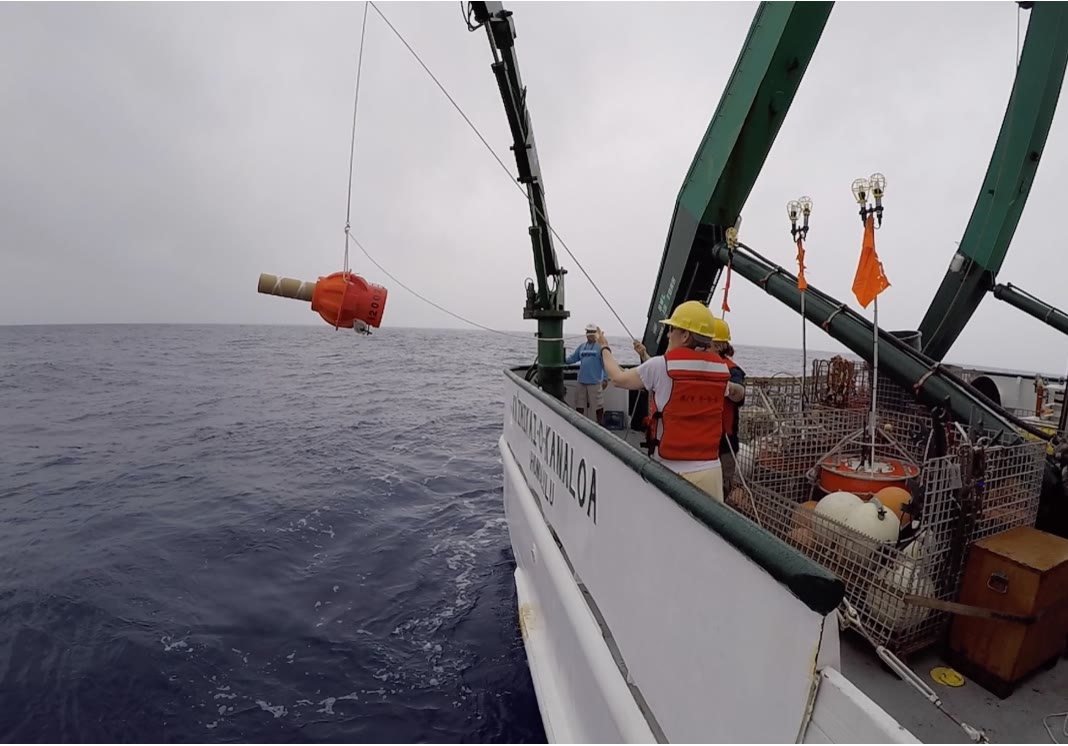
\includegraphics[width=0.6\linewidth]{images/book3/b1-deep-float.jpg}

{\small एक गहरे महासागर का प्रोफ़ाइलिंग फ़्लोट (क्रेन से लटका नारंगी उपकरण), 2018 में एक अनुसंधान पोत से उतारा जाता हुआ; छोड़े जाने पर वह अपनी कार्यकारी गहराई तक डूबता है और अपना डेटा भेजने के लिए नियमित अंतराल पर सतह पर आता है। (फ़ोटो: अज्ञात NOAA छायाकार, सार्वजनिक डोमेन, विकिमीडिया कॉमन्स के माध्यम से।)}
\label{fig:b1:ocean-circulation:float}
\end{omfigure}
% ledger: commons:deep-solo, noaa:argo-25

अधिक्रमण ऊष्मा भी ले जाता है। जो जल उत्तर जाता है गरम और लौटता है ठंडा होकर, उत्तर के वायुमंडल को ऊष्मा दे चुका होता है।

\begin{proposition}[अधिक्रमण द्वारा ले जाई गई ऊष्मा]\label{prop:b1:ocean-circulation:heat}
यदि आयतन-परिवहन $Q$ एक \omterm{def:b1:spherical-astronomy:geographic}{अक्षांश} को उत्तर की ओर \omterm{def:b1:fluid-envelopes-structure:potential-temperature}{विभव तापमान}
$\theta_1$ पर पार करता है और $\theta_2$ पर दक्षिण लौटता है, द्रव्यमान के शुद्ध परिवहन के बिना, तो अधिक्रमण उत्तर की ओर ऊष्मा फ़्लक्स ले जाता है:
\[
  H = \rho c_p\,Q\,(\theta_1 - \theta_2),
\]
जहाँ $c_p$ समुद्री जल की विशिष्ट ऊष्मा है।
\end{proposition}
% ledger: teos10:cp0

\begin{proof}
प्रति सेकंड द्रव्यमान $\rho Q$ उत्तर की ओर ऊष्मा-अंतर्वस्तु $\rho Q
c_p\theta_1$ ले जाते हुए पार करता है, तापमान के एक मनमाने शून्य से गिनी गई, और वही द्रव्यमान दक्षिण की ओर $\rho Q c_p\theta_2$ ले जाते हुए पार करता है। शुद्ध उत्तर-वाही फ़्लक्स उनका अंतर है; चूँकि दोनों द्रव्यमान बराबर हैं, मनमाना शून्य निरस्त हो जाता है, और परिणाम ऊष्मा का एक वास्तविक परिवहन है।
\end{proof}

उत्तरी अटलांटिक का एक मोटा बजट, W.~श्मिट्ज़ द्वारा, खाड़ी धारा को \qty{18}{\celsius} पर \qty{40}{\sverdrup} जल उत्तर ले जाता दिखाता है, जिसमें से
\qty{14}{\sverdrup} \qty{2}{\celsius} पर गहरे जल के रूप में दक्षिण लौटते हैं। $c_p =
\qty{3992}{J.kg^{-1}.K^{-1}}$ और $\rho = \qty{1027}{kg.m^{-3}}$ के साथ, यह अधिक्रमण $1027 \times 3992 \times \num{14e6} \times 16 = \qty{0.92e15}{W}$ ले जाता है, लगभग
\qty{0.9}{PW}, \ang{24} उ के उत्तर; सावधान आकलन \qty{1.2}{PW} देते हैं, वायुमंडल और महासागर द्वारा मिलकर ध्रुव की ओर ऊष्मा परिवहन का एक-चौथाई। इस ऊष्मा का अधिकांश उत्तरी अटलांटिक के उत्तरी भाग पर वायु को दिया जाता है, जो एक कारण है कि नॉर्वे, \ang{60} उ पर, उसी \omterm{def:b1:spherical-astronomy:geographic}{अक्षांश} पर दक्षिणी ग्रीनलैंड से कहीं अधिक गरम है।
% ledger: stewart:heat-conveyor, rapid:home, teos10:cp0 (computed in calc/ch29.py)

गहरा परिसंचरण धीमा है। यदि उत्तरी अटलांटिक में डूबते जल को अंटार्कटिक परिध्रुवीय धारा के रास्ते उत्तरी प्रशांत पहुँचने में लगभग एक हज़ार वर्ष लगते हैं, तो उसकी औसत गति लगभग \qty{1}{mm/s} है, धारा-मीटर द्वारा दर्ज परिवर्ती गहरी धाराओं से सौ गुना कम। इसलिए उसकी गति मापी नहीं, बल्कि अनुरेखकों से अनुमानित होती है: ट्रिटियम, जिसे 1950 के दशक के परमाणु परीक्षणों ने वायुमंडल में छोड़ा और जो 12.3 वर्ष की अर्ध-आयु से क्षय होता है, गहरे उत्तरी अटलांटिक में प्रविष्ट हुआ जहाँ गहरा जल बनता है, और 25 वर्षों के बाद \ang{30} उ के दक्षिण में बहुत कम फैला था, \qty{1}{mm/s} से कम की औसत गति। महासागर का आयतन, गहरे जल के बनने की दर से भाग दिया जाए, वही कोटि का समय देता है (\cref{exo:b1:ocean-circulation:12})।
% ledger: stewart:deep-circulation, nos:conveyor

अंटार्कटिक परिध्रुवीय धारा महासागरों को जोड़ती है। उसकी धाराएँ समुद्र-तल तक पहुँचती हैं और धीमी हैं, लगभग \qty{10}{cm/s}, और उसके मोर्चों पर \qty{50}{cm/s} तक, पर वह गहरी और चौड़ी है: दक्षिण अमेरिका और अंटार्कटिका के बीच ड्रेक पैसेज में मूरिंग धारा-मीटरों की एक सरणी ने \qty[uncertainty-mode=separate]{125 \pm 11}{\sverdrup} दिया (1985 में प्रकाशित), और 2007--2011 की एक घनी सरणी, जिसने तल के निकट की धाराएँ भी मापीं, \qty{173.3}{\sverdrup} दिया, उस लंबे समय से उपयोग किए गए मान से \qty{39}{\percent} अधिक। यह हर महासागर से जल को दूसरों तक ले जाता है और रास्ते में उसे मिलाता है।
% ledger: stewart:acc, donohue:acc

\begin{dated}{2021}
% ledger: ipcc:amoc-observed, ipcc:amoc-projected
जलवायु परिवर्तन पर अंतरसरकारी पैनल का 2021 का आकलन पुनर्निर्माणों से पाता है कि पिछले \num{8000} वर्षों में अटलांटिक अधिक्रमण अपेक्षाकृत स्थिर था (\emph{मध्यम विश्वास}), 19वीं शताब्दी के अंत में एक दुर्बलता के आरंभ के साथ (\emph{मध्यम विश्वास}), पर 20वीं शताब्दी में एक समग्र गिरावट के लिए केवल \emph{निम्न विश्वास} है। 2000 के दशक के मध्य से 2010 के दशक के मध्य तक सीधे प्रेक्षित दुर्बलता (\emph{उच्च विश्वास}) को दशक-पैमाने की परिवर्तनशीलता से अलग नहीं किया जा सकता (\emph{उच्च विश्वास})। अधिक्रमण सभी उत्सर्जन परिदृश्यों के लिए 21वीं शताब्दी में दुर्बल होने की \emph{अति संभावित} है, गिरावट के आकार में केवल \emph{निम्न विश्वास} के साथ; 2100 से पहले वह अचानक ध्वस्त नहीं होगा, इसका \emph{मध्यम विश्वास} है।
\end{dated}

\section{अभ्यास}

\begin{exercise}[$\star$]\label{exo:b1:ocean-circulation:1}
थोक सूत्र को $\rho_a = \qty{1.3}{kg.m^{-3}}$ और येलैंड और टेलर के खिंचाव-गुणांक के साथ लें।
(क)~$C_D$ और \omterm{def:b1:ocean-circulation:wind-stress}{पवन-प्रतिबल} परिकलित करें, 4, 7 और \qty{15}{m/s} की पवनों के लिए। (ख)~\qty{7}{m/s} से \qty{15}{m/s} तक प्रतिबल किस गुणक से बढ़ता है? उसकी तुलना गतियों के वर्गों के अनुपात से करें और अंतर समझाएँ।
% ledger: stewart:wind-stress, stewart:drag-coefficient
\end{exercise}

\begin{exercise}[$\star$]\label{exo:b1:ocean-circulation:2}
हर स्थिति में \omterm{def:b1:ocean-circulation:ekman}{एकमान परिवहन} की दिशा दें। (क)~\ang{45} उ पर पूर्व की ओर बहती पवन। (ख)~\ang{15} उ पर उत्तर-पूर्व से एक व्यापारिक पवन।
(ग)~\ang{50} द पर पूर्व की ओर बहती पवन। (घ)~दक्षिणी अफ़्रीका के पश्चिमी तट के साथ, \ang{23} द के निकट, दक्षिण से एक पवन। चारों में से किस स्थिति में परिवहन तट से दूर इंगित करता है, और उसके बाद क्या होता है?
\end{exercise}

\begin{exercise}[$\star$]\label{exo:b1:ocean-circulation:3}
\ang{26.5} उ पर अटलांटिक में, 2004--2024 के माध्य परिवहन हैं: फ़्लोरिडा जलडमरूमध्य \qty{31.7}{\sverdrup}, एकमान \qty{3.5}{\sverdrup}, ऊपरी मध्य-महासागर \qty{-17.9}{\sverdrup}; परतों के अनुसार, 0--\qty{800}{m} \qty{16.6}{\sverdrup}, 800--\qty{1100}{m} \qty{0.4}{\sverdrup}, 1100--\qty{3000}{m} \qty{-12.0}{\sverdrup}, 3000--\qty{5000}{m} \qty{-5.9}{\sverdrup} (उत्तर की ओर धनात्मक)। (क)~पहले तीन जोड़ें और प्रकाशित अधिक्रमण, \qty{17.1}{\sverdrup} से तुलना करें। (ख)~\qty{1100}{m} के ऊपर के उत्तर-वाही प्रवाह की नीचे के दक्षिण-वाही प्रवाह से तुलना करें। (ग)~\qty{17.1}{\sverdrup} को घन किलोमीटर प्रति वर्ष में बदलें, और वह समय परिकलित करें जो यह प्रवाह पूरे महासागर का आयतन, \qty{1.3324e9}{km^3}, भरने में लेगा।
% ledger: rapid:transports, charette:ocean-volume
\end{exercise}

\begin{exercise}[$\star$]\label{exo:b1:ocean-circulation:4}
एकमान के सूत्रों से, \qty{10}{m/s} की पवन के नीचे \ang{15}, \ang{45} और \ang{60} \omterm{def:b1:spherical-astronomy:geographic}{अक्षांश} पर एकमान गहराई और सतही धारा परिकलित करें, और सतही धारा को पवन के प्रतिशत के रूप में। सूत्र भूमध्य रेखा के निकट क्यों विफल होते हैं?
% ledger: stewart:ekman-constants
\end{exercise}

\begin{exercise}[$\star\star$]\label{exo:b1:ocean-circulation:5}
\ang{11} उ पर अटलांटिक में, \qty{5000}{km} चौड़ाई पर पश्चिम की ओर \qty{0.07}{Pa} का माध्य \omterm{def:b1:ocean-circulation:wind-stress}{पवन-प्रतिबल} लें, और
$\rho = \qty{1027}{kg.m^{-3}}$।
(क)~प्रति मीटर \omterm{def:b1:ocean-circulation:ekman}{एकमान परिवहन} और उसकी दिशा परिकलित करें। (ख)~खंड के आर-पार कुल आयतन-परिवहन \omterm{def:b1:ocean-circulation:ekman}{स्वर्डरप} में परिकलित करें। (ग)~उसकी तुलना प्रत्यक्ष मापे गए परिवहनों ($12.0 \pm \qty{5.5}{\sverdrup}$) और दीर्घकालीन पवनों से परिकलित ($13.5 \pm \qty{0.3}{\sverdrup}$) से करें।
% ledger: stewart:ekman-transport
\end{exercise}

\begin{exercise}[$\star\star$]\label{exo:b1:ocean-circulation:6}
भूमध्यरेखीय प्रशांत पर \omterm{def:b1:atmospheric-circulation:winds}{व्यापारिक पवनें} पश्चिम की ओर \qty{0.05}{Pa} का प्रतिबल लगाती हैं।
(क)~प्रति मीटर \omterm{def:b1:ocean-circulation:ekman}{एकमान परिवहन} और उसकी दिशा परिकलित करें, \ang{2} उ और \ang{2}~द पर। (ख)~मान लें कि इन दोनों अक्षांशों के आर-पार दूर ले जाया गया जल उनके बीच नीचे से बदला जाता है, तो औसत \omterm{def:b1:ocean-circulation:upwelling}{उत्सर्पण} वेग प्रति दिन मीटर में परिकलित करें। (ग)~प्रमेय के सूत्र का भूमध्य रेखा पर स्वयं क्या होता है? कौन-सा निष्कर्ष बचता है?
\end{exercise}

\begin{exercise}[$\star\star$]\label{exo:b1:ocean-circulation:7}
एक \omterm{def:b1:ocean-circulation:gyre}{उपोष्णकटिबंधीय गायर} पर, \ang{15} उ पर पश्चिम की ओर \qty{0.06}{Pa} और \ang{40} उ पर पूर्व की ओर \qty{0.12}{Pa} का \omterm{def:b1:ocean-circulation:wind-stress}{पवन-प्रतिबल} लें। (क)~दोनों \omterm{def:b1:ocean-circulation:ekman}{एकमान परिवहन} और उनकी दिशाएँ परिकलित करें। (ख)~मान लें कि दोनों अक्षांशों के बीच परिवहन समान रूप से बदलता है, तो \omterm{def:b1:ocean-circulation:ekman}{एकमान परत} के आधार पर ऊर्ध्वाधर वेग प्रति वर्ष मीटर में परिकलित करें, और कहें कि वह ऊपर है या नीचे। (ग)~\qty{5000}{km} चौड़े बेसिन पर, परत के आधार से कितने \omterm{def:b1:ocean-circulation:ekman}{स्वर्डरप} पंप होते हैं?
\end{exercise}

\begin{exercise}[$\star\star$]\label{exo:b1:ocean-circulation:8}
$\rho = \qty{1027}{kg.m^{-3}}$ और $c_p = \qty{3992}{J.kg^{-1}.K^{-1}}$ लें।
(क)~\qty{15}{\celsius} पर उत्तर की ओर बहते और \qty{3}{\celsius} पर लौटते \qty{17}{\sverdrup} द्वारा उत्तर ले जाई गई ऊष्मा परिकलित करें। (ख)~उसकी तुलना अटलांटिक अधिक्रमण द्वारा ले जाए गए \qty{1.2}{PW} से करें। (ग)~यदि वही जल सतह पर \qty{12}{\celsius} पर, बेसिन के पूर्वी ओर के साथ, दक्षिण लौटता, तो वह कितनी ऊष्मा ले जाता? इससे गहरे जल के निर्माण के महत्व के बारे में क्या पता चलता है?
% ledger: rapid:home, teos10:cp0
\end{exercise}

\begin{exercise}[$\star\star$]\label{exo:b1:ocean-circulation:9}
दक्षिणी अटलांटिक के तीन जल-द्रव्यमानों के \omterm{def:b1:fluid-envelopes-structure:potential-temperature}{विभव तापमान} और लवणताएँ हैं: अंटार्कटिक मध्यवर्ती जल \qty{3.3}{\celsius}, 34.15; उत्तरी अटलांटिक गहरा जल \qty{4.0}{\celsius}, 35.00; अंटार्कटिक तल-जल \qty{0.4}{\celsius},
34.67। गहराई पर एक नमूने का $\theta = \qty{2.78}{\celsius}$ और $S = 34.731$ है। \cref{prop:b1:fluid-envelopes-structure:mixing} का उपयोग करके, नमूने में हर \omterm{def:b1:fluid-envelopes-structure:ts-diagram}{जल-द्रव्यमान} का अंश ज्ञात करें।
% ledger: stewart:deep-circulation
\end{exercise}

\begin{exercise}[$\star\star\star$]\label{exo:b1:ocean-circulation:10}
\cref{prop:b1:ocean-circulation:spiral} के सर्पिल को लें। (क)~दिखाएँ कि $u$ और $v$ संतुष्ट करते हैं $f v + A_z u'' = 0$ और $-f u + A_z v'' = 0$।
(संकेत: लिखें $u + iv =
V_0\,e^{i\pi/4}\,e^{(1+i)az}$।) (ख)~दिखाएँ कि सतह पर प्रतिबल $\rho A_z\,\partial\vec
v/\partial z$ \omterm{def:b1:ocean-circulation:wind-stress}{पवन-प्रतिबल} $(0, T)$ के बराबर है। (ग)~परिवहन $\int_{-\infty}^0 \rho u\,\mathrm dz$ और $\int_{-\infty}^0 \rho
v\,\mathrm dz$ परिकलित करें, और जाँचें कि वे \cref{thm:b1:ocean-circulation:ekman} से मेल खाते हैं।
\end{exercise}

\begin{exercise}[$\star\star\star$]\label{exo:b1:ocean-circulation:11}
स्टॉमेल के मॉडल में, \omterm{def:b1:ocean-circulation:wbc}{पश्चिमी सीमा धारा} की चौड़ाई लगभग $R/\beta$ है,
जहाँ $R$ तल-घर्षण की दर है और $\beta = \mathrm df/\mathrm dy$ \omterm{def:b1:atmospheric-circulation:coriolis-parameter}{कोरिऑलिस प्राचल} की उत्तर की ओर वृद्धि-दर है। (क)~दिखाएँ कि $\beta = 2\Omega
\cos\varphi/a_\oplus$ है और \ang{30} उ पर ($a_\oplus = \qty{6371}{km}$) उसे परिकलित करें।
(ख)~$R = \qty{e-6}{s^{-1}}$ के साथ चौड़ाई परिकलित करें। (ग)~\qty{30}{\sverdrup} का परिवहन \qty{5000}{km} चौड़े बेसिन के अंदरूनी भाग के आर-पार ऊपरी \qty{1000}{m} में दक्षिण की ओर अपवाहित होता है, और उसी गहराई पर \omterm{def:b1:ocean-circulation:wbc}{पश्चिमी सीमा धारा} में उत्तर लौटता है। दोनों औसत गतियाँ परिकलित करें और उनकी तुलना खाड़ी धारा की गति, \qty{1.8}{m/s} से करें।
% ledger: stewart:north-atlantic, nos:gulf-stream, earth:Rmean
\end{exercise}

\begin{exercise}[$\star\star\star$]\label{exo:b1:ocean-circulation:12}
महासागर \qty{1.3324e9}{km^3} रखता है, \qty{361.84e6}{km^2} पर फैला हुआ। (क)~दिखाएँ कि \qty{1000}{m} के नीचे का आयतन कम से कम \qty{9.71e8}{km^3} है। (ख)~उत्तरी अटलांटिक गहरा जल लगभग \qty{17}{\sverdrup} पर और अंटार्कटिक तल-जल लगभग \qty{9}{\sverdrup} पर बनता है। \qty{1000}{m} के नीचे का जल नवीकृत होने में लगने वाला समय आकलित करें, और उसे संवाहक के हज़ार वर्षों से तुलना करें। (ग)~ट्रिटियम की अर्ध-आयु 12.3 वर्ष है। 25 वर्षों के बाद एक ट्रिटियम इनपुट का कितना अंश बचता है? \qty{1}{mm/s} पर चलता जल 25 वर्षों में कितनी दूर जाता है?
% ledger: charette:ocean-volume, stewart:deep-circulation, stewart:acc, rapid:transports
\end{exercise}

\section{समस्या: एक उत्सर्पण तट}

\begin{problem}[{सप्ताहांत समस्या --- \ang{38} उ पर एक ग्रीष्मकालीन पवन, एक तट के साथ}]
\label{pb:b1:ocean-circulation:1}
% values: calc/ch29.py (invented coast; constants from the ledger)
एक सीधा तट \ang{38} उ पर उत्तर-दक्षिण चलता है, जिसका महासागर पश्चिम में है। ग्रीष्म में, \qty{8}{m/s} की एक स्थायी पवन हफ़्तों तक उसके साथ उत्तर से बहती है। तट काल्पनिक है, पर उसकी संख्याएँ समुद्रों की पूर्वी ओर के विशिष्ट मान हैं।
उपयोग करें $\Omega = 2\pi/(\qty{23.9345}{h})$, $\rho_a = \qty{1.3}{kg.m^{-3}}$, येलैंड और टेलर का खिंचाव-गुणांक, समुद्री जल के लिए $\rho = \qty{1027}{kg.m^{-3}}$ और $c_p = \qty{3992}{J.kg^{-1}.K^{-1}}$।

\medskip
\noindent\textbf{भाग I --- पवन और उसका प्रतिबल।}
\begin{enumerate}
  \item पवन किस दिशा में बहती है? क्या वह तट के साथ है या उसके आर-पार?
  \item खिंचाव-गुणांक परिकलित करें।
  \item \omterm{def:b1:ocean-circulation:wind-stress}{पवन-प्रतिबल} परिकलित करें।
  \item \qty{12}{m/s} की पवन के लिए वही दो प्रश्न। प्रतिबल किस गुणक से बढ़ता है, और वह गतियों के वर्गों के अनुपात से अधिक क्यों है?
  \item \ang{38} उ पर \omterm{def:b1:atmospheric-circulation:coriolis-parameter}{कोरिऑलिस प्राचल} परिकलित करें।
  \item $2\pi/f$ घंटों में परिकलित करें। एकमान संतुलन लागू होने से पहले पवन एक दिन या अधिक क्यों बहनी चाहिए?
\end{enumerate}

\medskip
\noindent\textbf{भाग II --- एकमान परत।}
\begin{enumerate}[resume]
  \item \omterm{def:b1:ocean-circulation:ekman}{एकमान परिवहन} किस दिशा में है? भूमि की ओर या खुले समुद्र की ओर?
  \item तट के प्रति मीटर एकमान द्रव्यमान परिवहन परिकलित करें।
  \item उसे प्रति मीटर आयतन-परिवहन में बदलें।
  \item एकमान के सूत्र से एकमान गहराई परिकलित करें।
  \item परत में औसत अपतटीय वेग परिकलित करें, \unit{cm/s} में।
  \item एकमान के सूत्र से सतही धारा और उसकी दिशा परिकलित करें। ड्रिफ़्टर मापन उसकी गति के बारे में इसके बजाय क्या सुझाते हैं?
\end{enumerate}

\medskip
\noindent\textbf{भाग III --- तट पर उत्सर्पण।}
\begin{enumerate}[resume]
  \item एक ऊर्ध्वाधर परिच्छेद के रेखाचित्र से समझाएँ कि अपतटीय ले जाया गया जल कहाँ से आता है।
  \item तट के हर किलोमीटर के साथ प्रति दिन उत्सर्पित आयतन परिकलित करें।
  \item मान लें जल तट के साथ \qty{20}{km} चौड़ी पट्टी से ऊपर उठता है। माध्य ऊर्ध्वाधर वेग परिकलित करें, \unit{m/s} में और मीटर प्रति दिन में।
  \item इस गति से \omterm{def:b1:ocean-circulation:ekman}{एकमान परत} के आधार से सतह तक ऊपर उठने में जल को कितना समय लगता है?
  \item उत्सर्पित जल \qty{12}{\celsius} पर सतह तक पहुँचता है, जबकि अपतटीय खुला समुद्र \qty{18}{\celsius} पर है। समुद्री पवन अपतटीय गरम, नम वायु को इस जल पर ले जाती है। सतह के निकट वायु का क्या होता है, और तट पर कौन-सा मौसम आता है?
  \item ऐसे तट मछलियों से समृद्ध क्यों हैं?
  \item शरद में पवन पलटती है और एक सप्ताह दक्षिण से बहती है। परिवहन और तट पर जल का क्या होता है?
\end{enumerate}

\medskip
\noindent\textbf{भाग IV --- अन्य तट और कुल परिवहन।}
\begin{enumerate}[resume]
  \item वही प्रतिबल के साथ, \ang{20} उ पर तट के प्रति मीटर \omterm{def:b1:ocean-circulation:ekman}{एकमान परिवहन} परिकलित करें और \ang{38} उ से तुलना करें।
  \item दक्षिणी अफ़्रीका के पश्चिमी तट पर, \ang{23} द के निकट, कौन-सी पवन-दिशा \omterm{def:b1:ocean-circulation:upwelling}{उत्सर्पण} चलाती है? समस्या के तट से तुलना करें।
  \item \ang{38} उ पर \qty{8}{m/s} के बजाय \qty{5}{m/s} की पवन के नीचे प्रतिबल और प्रति मीटर \omterm{def:b1:ocean-circulation:ekman}{एकमान परिवहन} परिकलित करें, और प्रश्न~8 के मानों से उनका अनुपात।
  \item उत्सर्पित जल अपतटीय बहते हुए \qty{6}{\celsius} गरम होता है। तट के प्रति मीटर प्रति सेकंड, फिर \qty{1000}{km} के साथ, उसकी ली गई ऊष्मा परिकलित करें।
  \item ऐसे तट की कितनी लंबाई उतना जल उत्सर्पित करेगी जितना खाड़ी धारा फ़्लोरिडा जलडमरूमध्य से \qty{31.7}{\sverdrup} ले जाती है?
  \item इस तट के \qty{1000}{km} के साथ उत्सर्पित जल का आयतन, \omterm{def:b1:ocean-circulation:ekman}{स्वर्डरप} में, कितना है?
\end{enumerate}
\end{problem}
